\documentclass[11pt]{article}
\usepackage{subfigure,wrapfig,booktabs,fancyhdr,amsmath,amsfonts,float}
\usepackage[pdftex]{graphicx}
\usepackage{bm,amssymb,amsmath,amsthm,wasysym,color,fullpage,setspace,multirow}
\usepackage{listings}
\lstset{language=Matlab}

\newcommand{\vb}{\boldsymbol}
\newcommand{\vbh}[1]{\hat{\boldsymbol{#1}}}
\newcommand{\vbb}[1]{\bar{\boldsymbol{#1}}}
\newcommand{\vbt}[1]{\tilde{\boldsymbol{#1}}}
\newcommand{\vbs}[1]{{\boldsymbol{#1}}^*}
\newcommand{\vbd}[1]{\dot{{\boldsymbol{#1}}}}
\newcommand{\vbdd}[1]{\ddot{{\boldsymbol{#1}}}}
\newcommand{\by}{\times}
\newcommand{\tr}{{\rm tr}}
\newcommand{\cpe}[1]{\left[{#1} \times \right]}
\newcommand{\sfrac}[2]{\textstyle \frac{#1}{#2}}
\newcommand{\ba}{\begin{array}}
\newcommand{\ea}{\end{array}}
\renewcommand{\earth}{\oplus}
\newcommand{\sinc}{{\rm \hspace{0.5mm} sinc}}
\newcommand{\tf}{\tilde{f}}
\newcommand{\tbox}[1]{\noindent \fbox{\parbox{\textwidth}{#1}}}
\DeclareMathAlphabet{\mathpzc}{OT1}{pzc}{m}{it}

% Weird thing I have to add to allow `rubber` to compile
\DeclareUnicodeCharacter{2212}{-}

\title{ASE 389P-7 \\ Exam 2}
\author{Alejandro Moreno}\date{November 8, 2022}

\begin{document}
%\onehalfspace
\maketitle

\newpage
\section{Problem 4}

\subsection{a}

\begin{figure}[H]
	\centering
	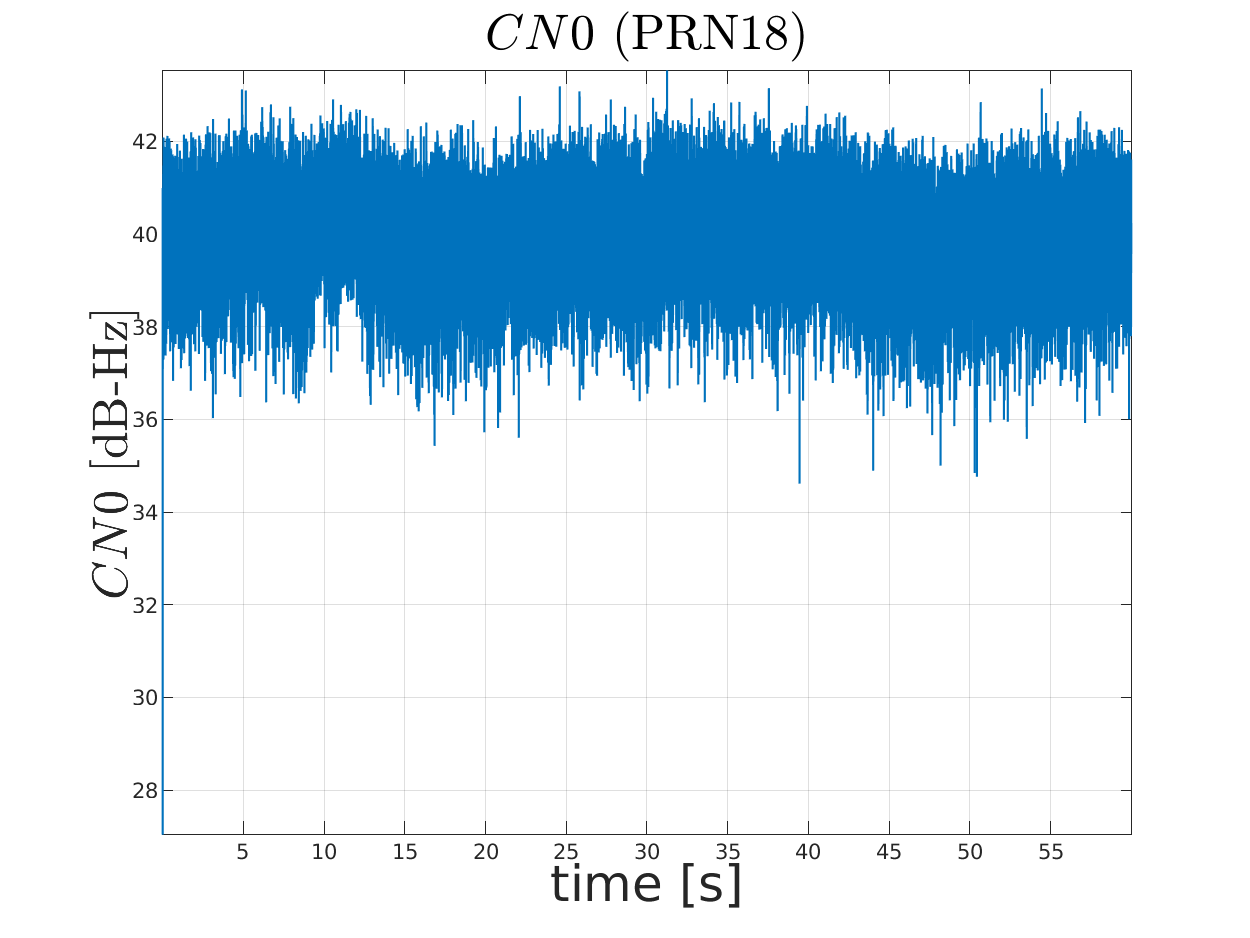
\includegraphics[width=0.9\textwidth]{fig/CN0_PRN18.png}
\end{figure}

\begin{figure}[H]
	\centering
	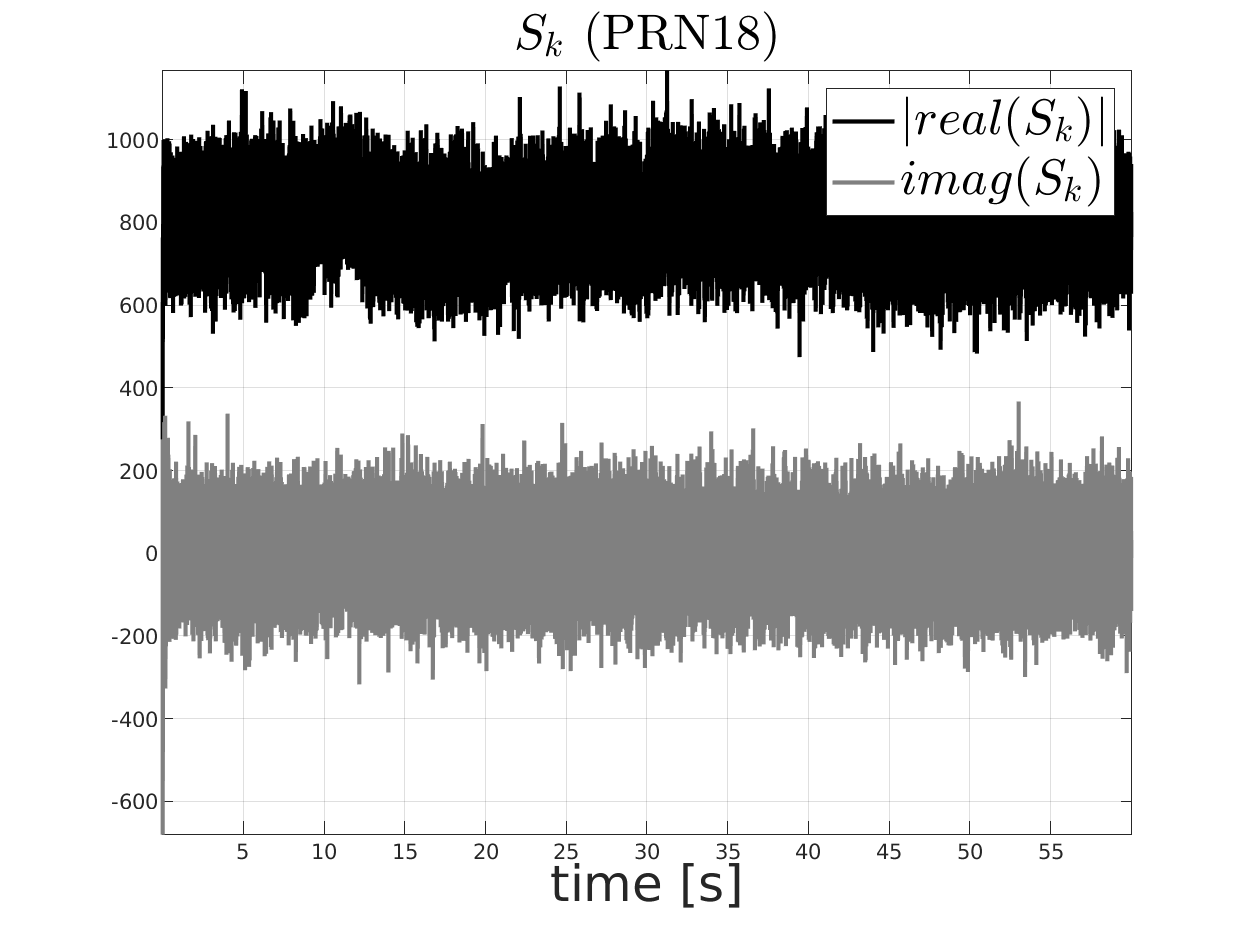
\includegraphics[width=0.9\textwidth]{fig/sk_PRN18.png}
\end{figure}

\begin{figure}[H]
	\centering
	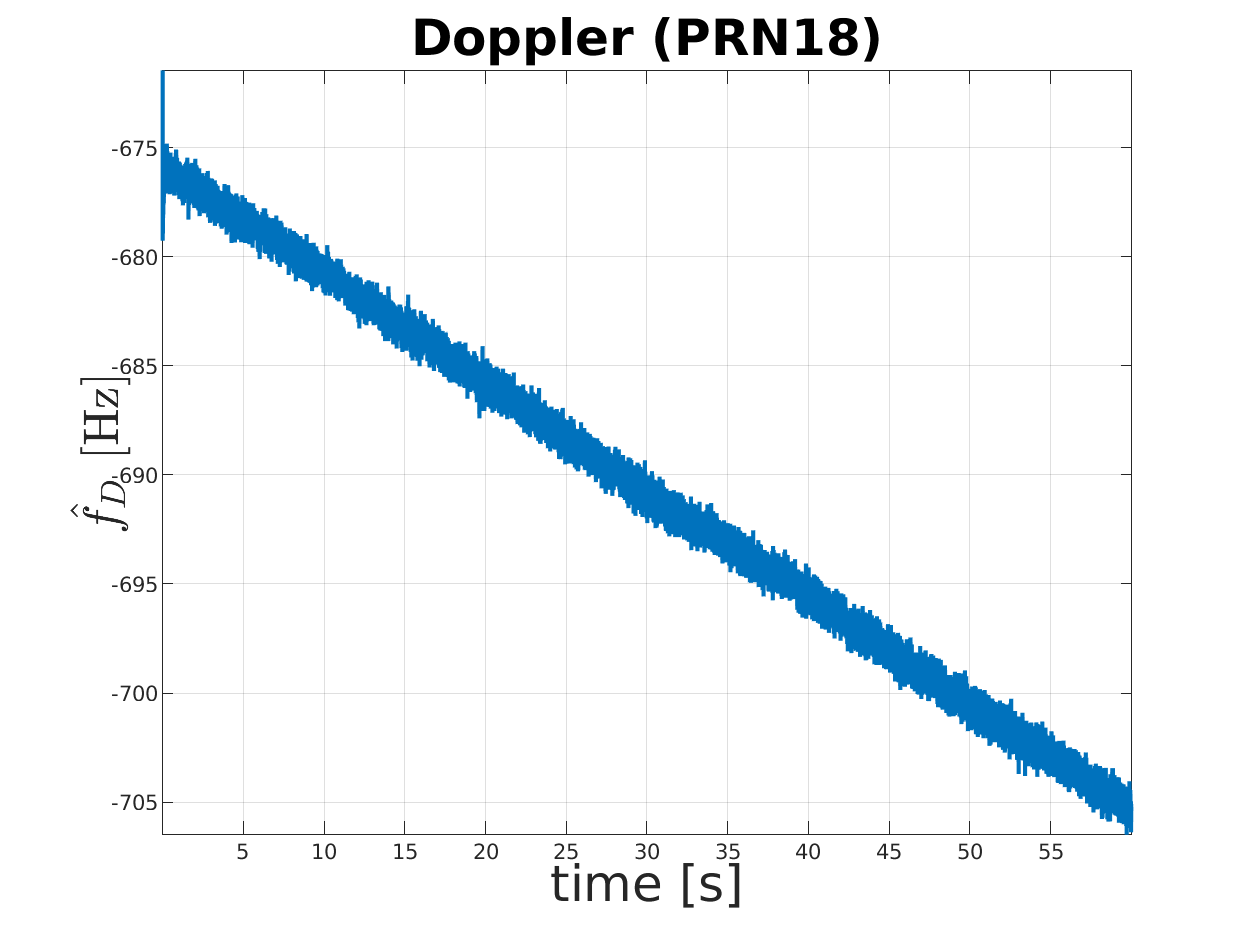
\includegraphics[width=0.9\textwidth]{fig/doppler_PRN18.png}
\end{figure}


\subsection{b}

%------------ PRN 10
\begin{figure}[H]
	\centering
	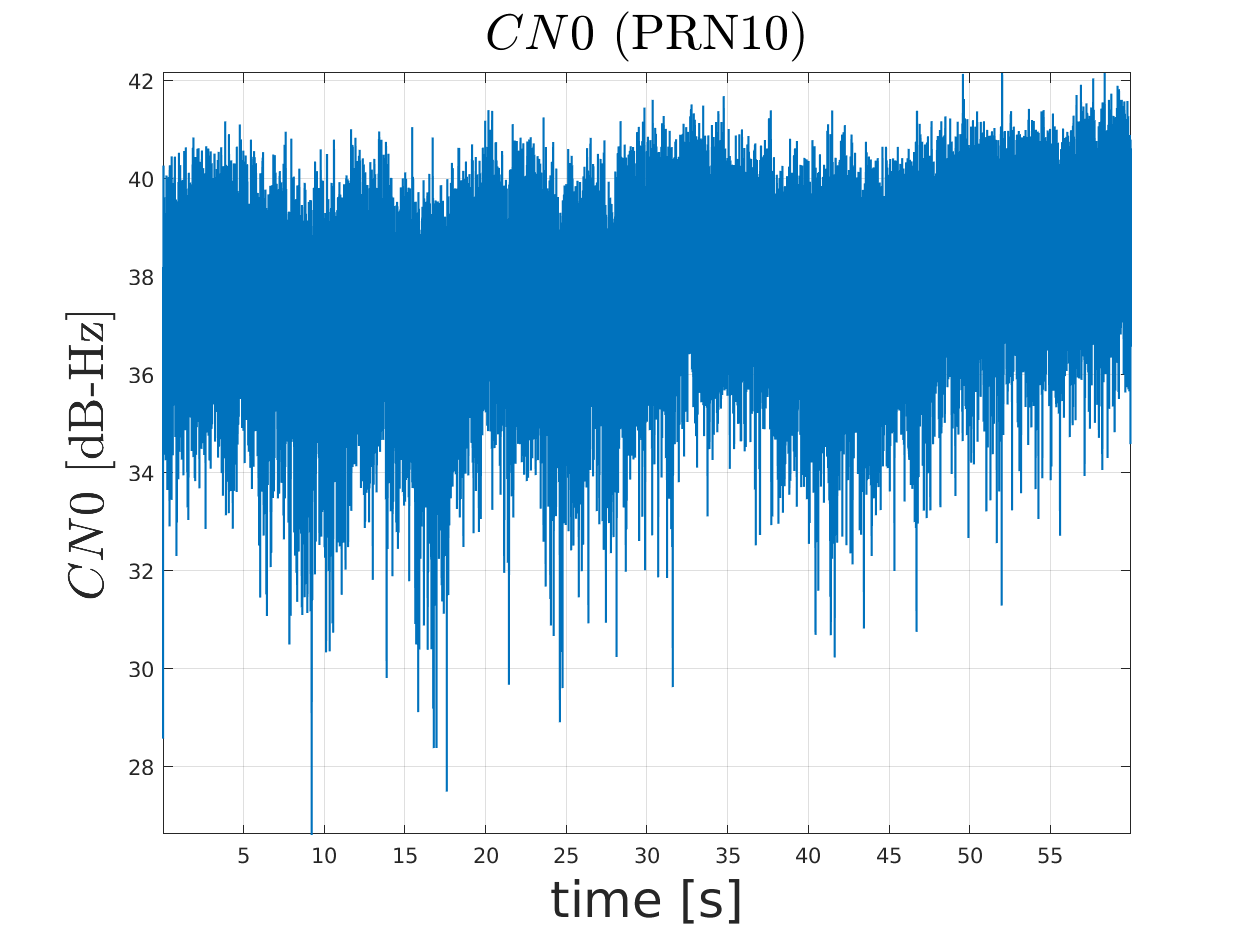
\includegraphics[width=0.9\textwidth]{fig/CN0_PRN10.png}
\end{figure}

\begin{figure}[H]
	\centering
	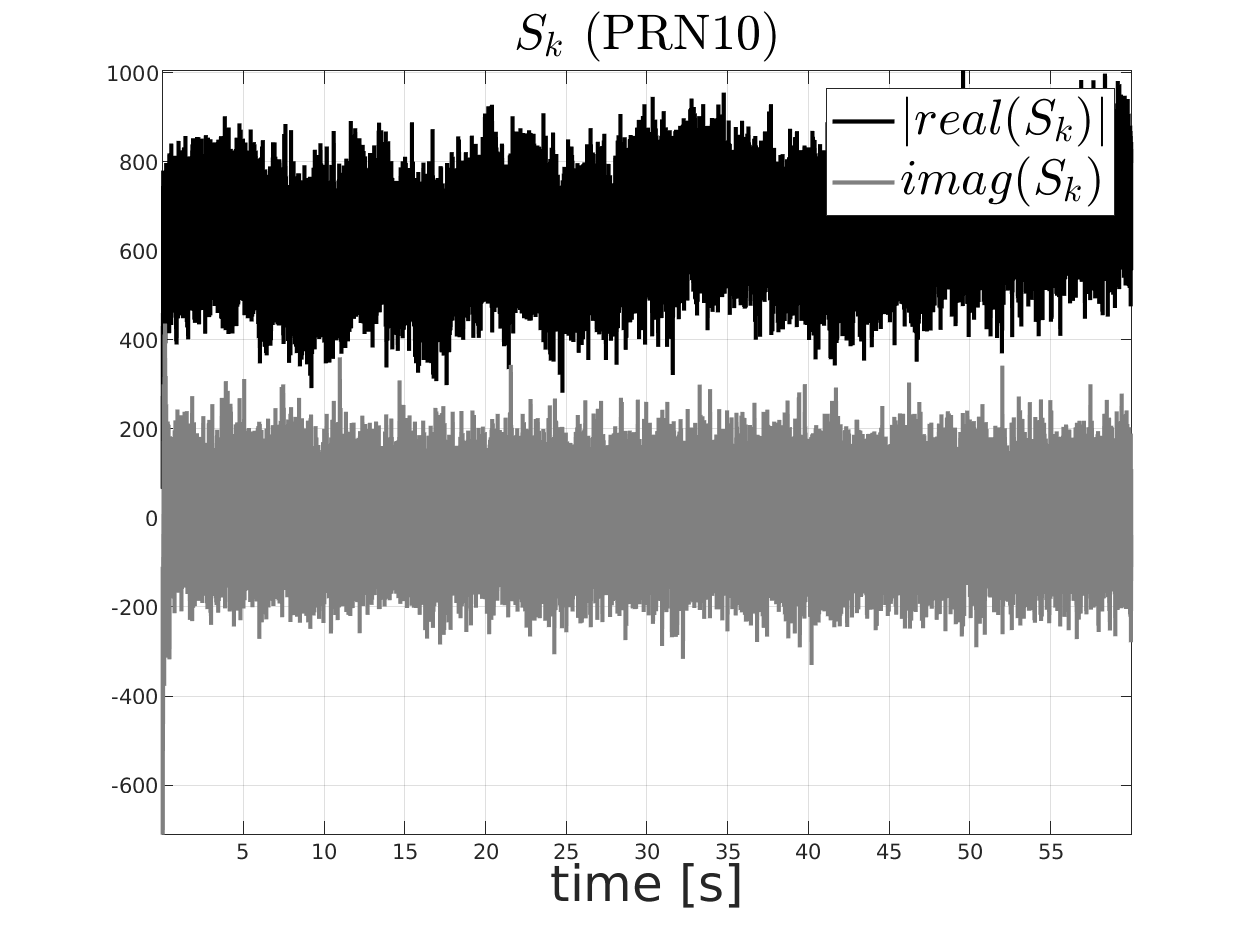
\includegraphics[width=0.9\textwidth]{fig/sk_PRN10.png}
\end{figure}

\begin{figure}[H]
	\centering
	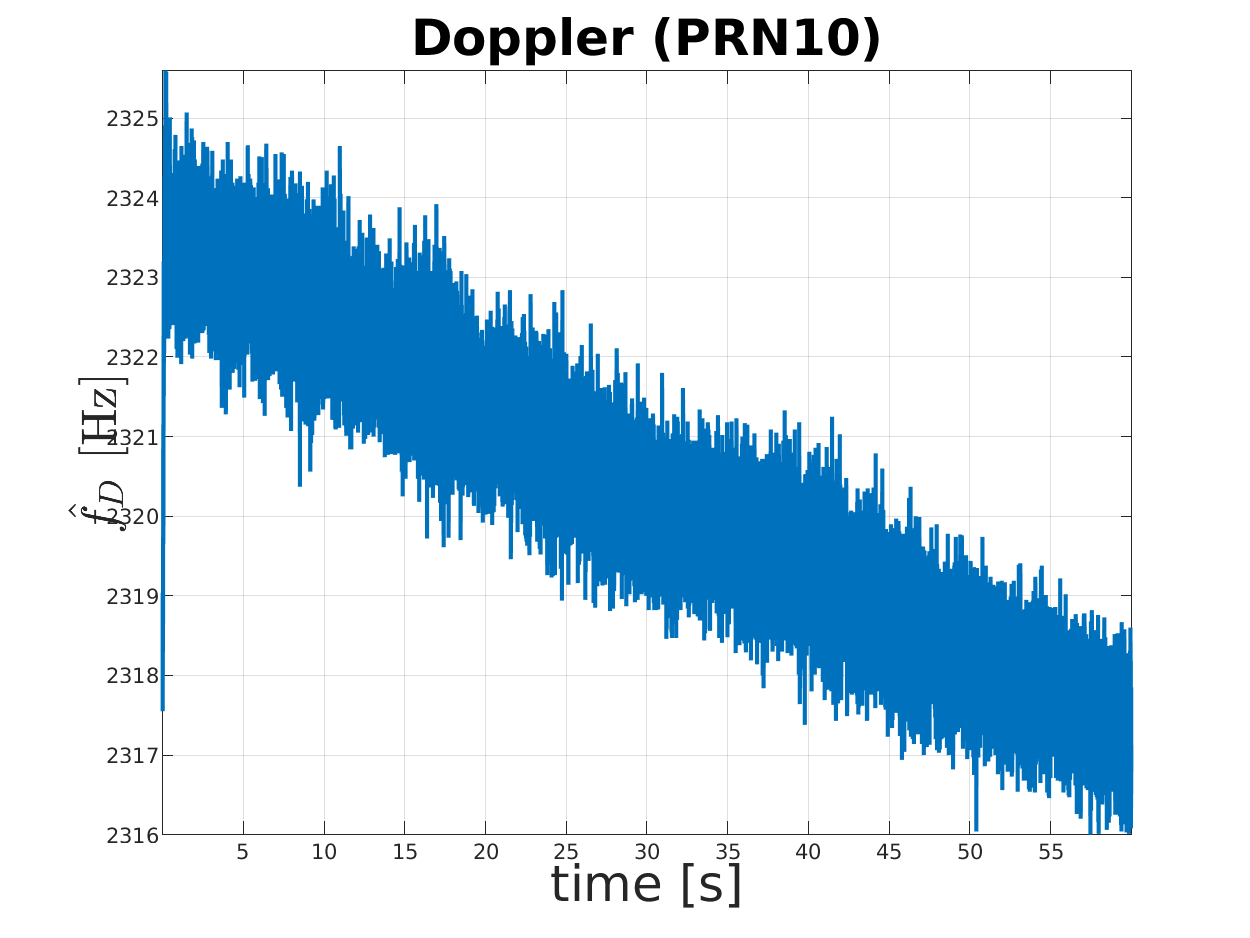
\includegraphics[width=0.9\textwidth]{fig/doppler_PRN10.png}
\end{figure}

%-------------- PRN 20
\begin{figure}[H]
	\centering
	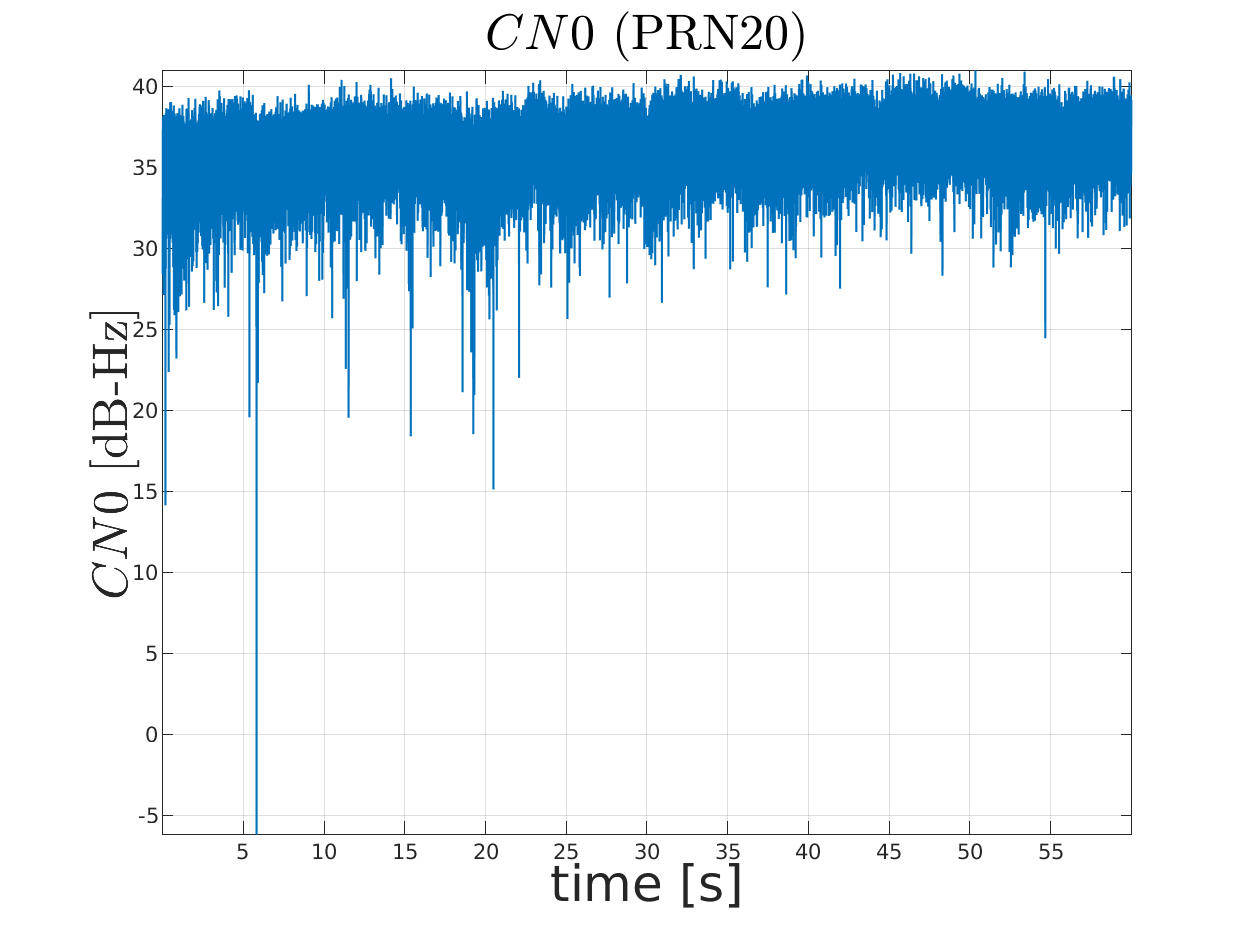
\includegraphics[width=0.9\textwidth]{fig/CN0_PRN20.png}
\end{figure}

\begin{figure}[H]
	\centering
	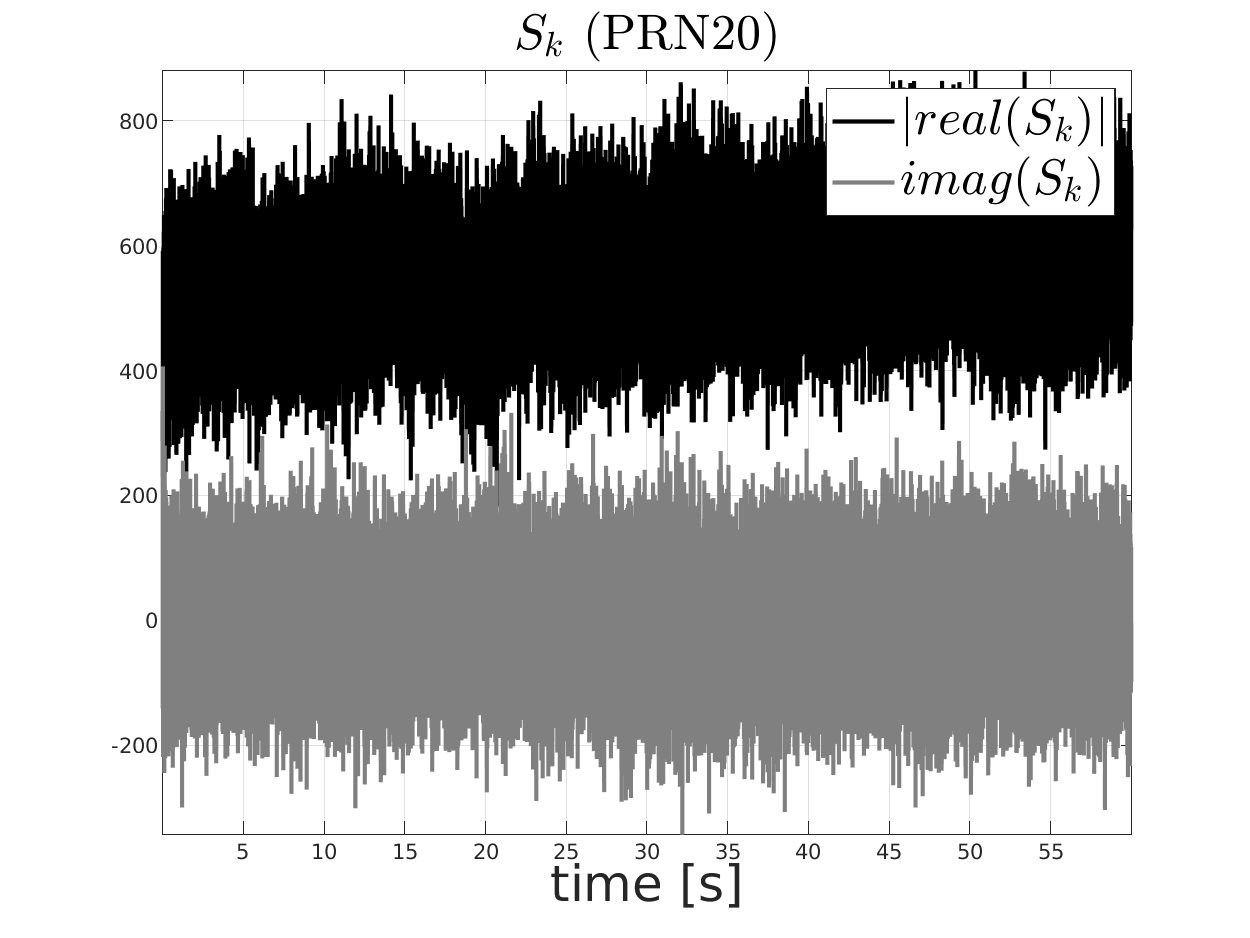
\includegraphics[width=0.9\textwidth]{fig/sk_PRN20.png}
\end{figure}

\begin{figure}[H]
	\centering
	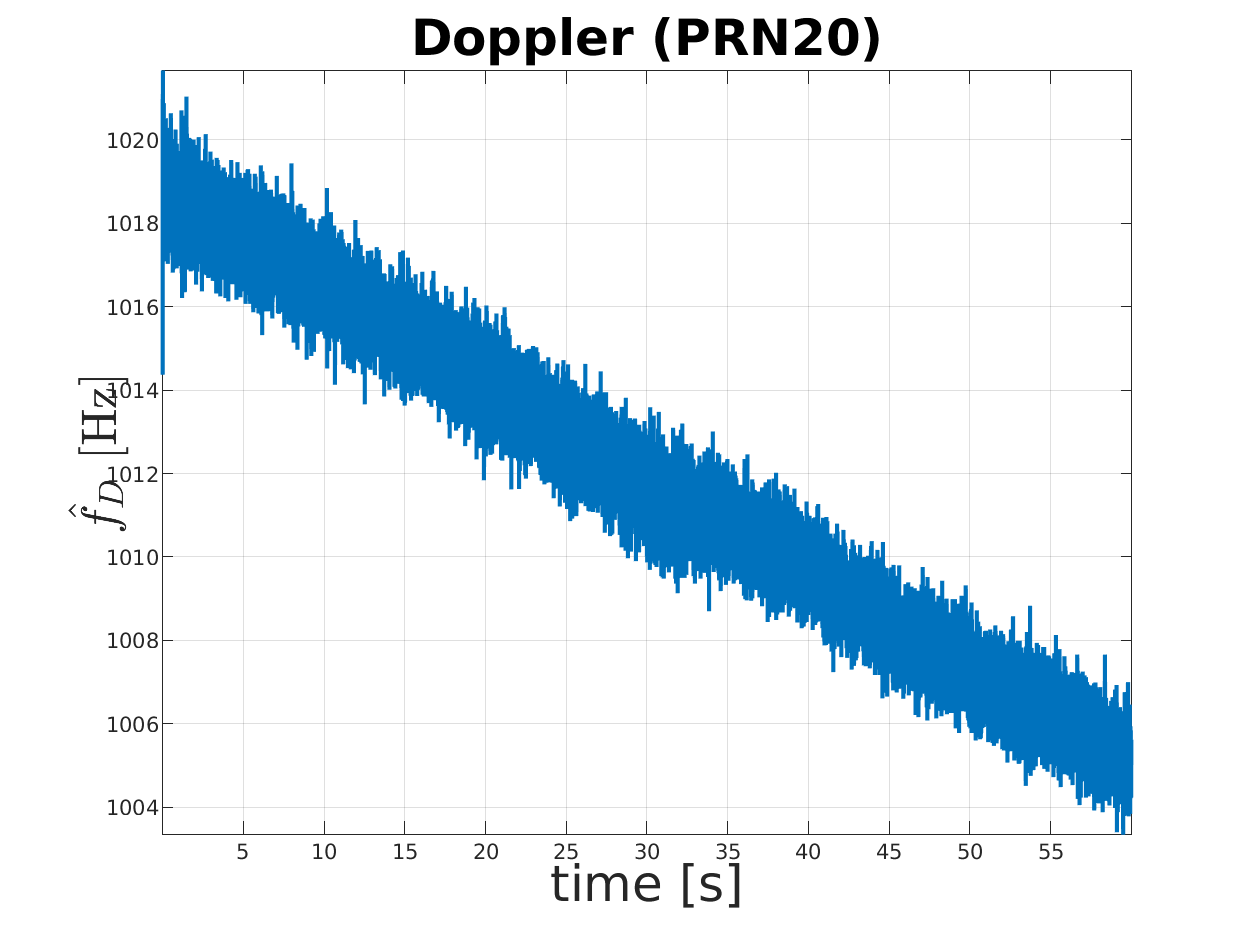
\includegraphics[width=0.9\textwidth]{fig/doppler_PRN20.png}
\end{figure}

%-------------- PRN 23
\begin{figure}[H]
	\centering
	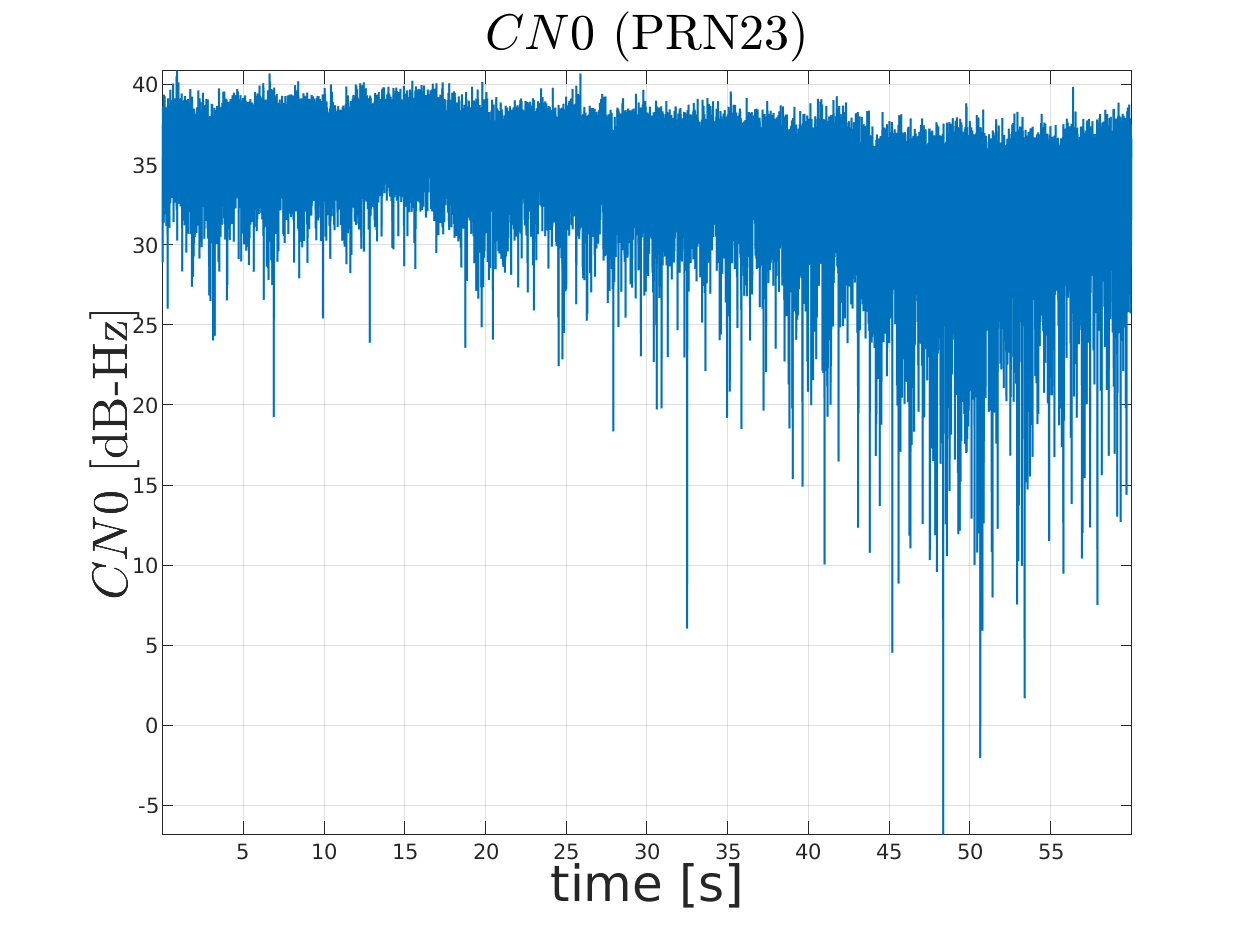
\includegraphics[width=0.9\textwidth]{fig/CN0_PRN23.png}
\end{figure}

\begin{figure}[H]
	\centering
	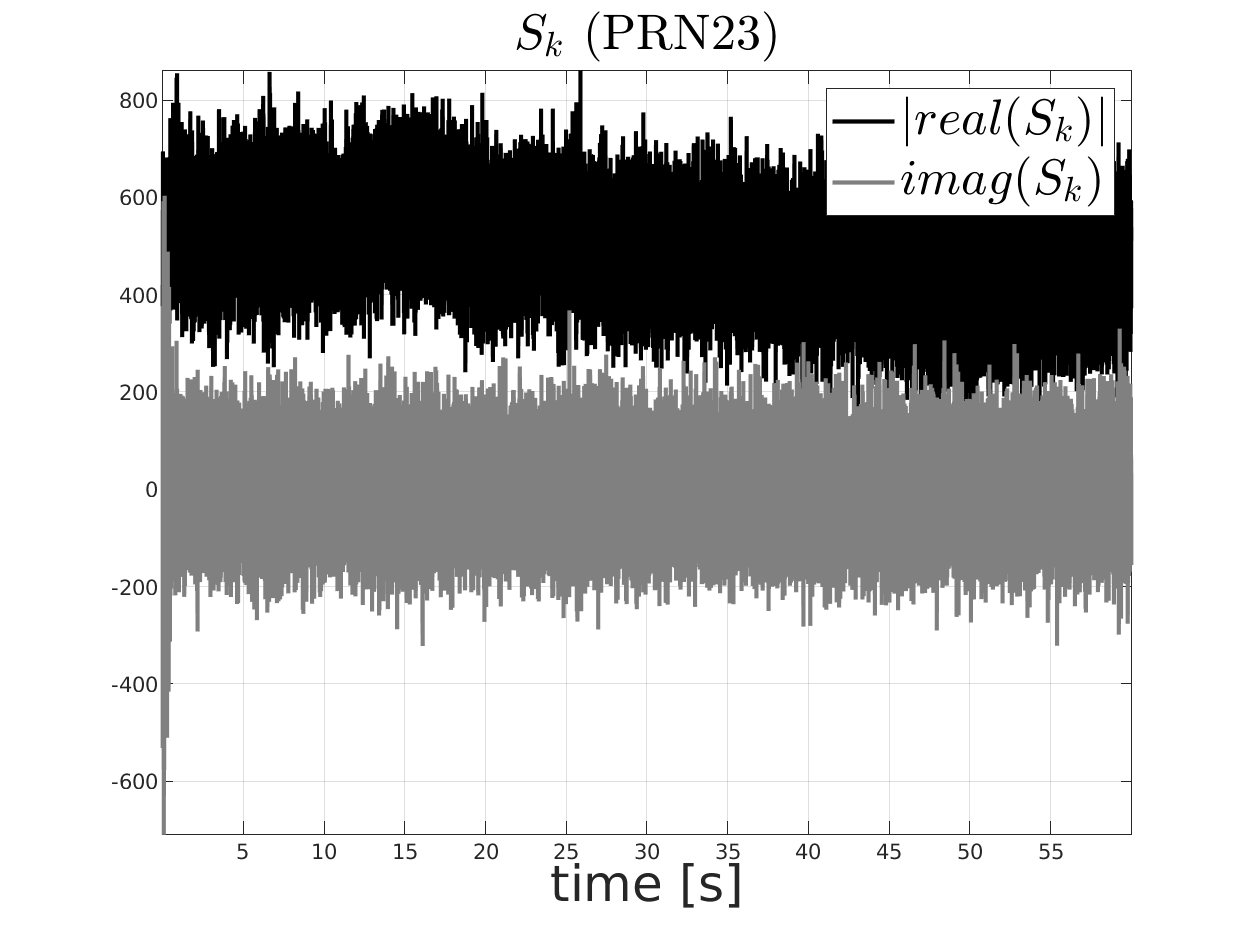
\includegraphics[width=0.9\textwidth]{fig/sk_PRN23.png}
\end{figure}

\begin{figure}[H]
	\centering
	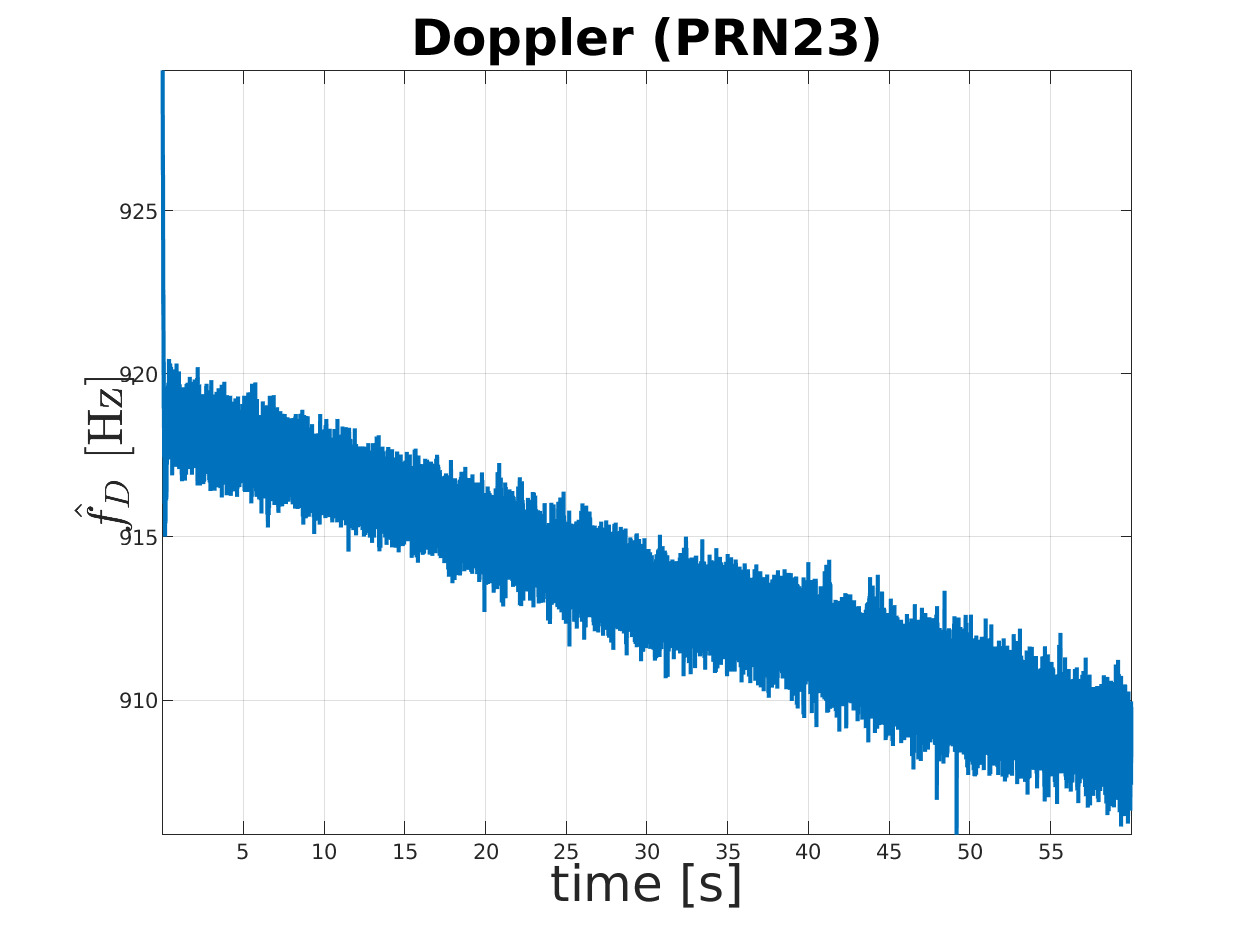
\includegraphics[width=0.9\textwidth]{fig/doppler_PRN23.png}
\end{figure}

%-------------- PRN 24
\begin{figure}[H]
	\centering
	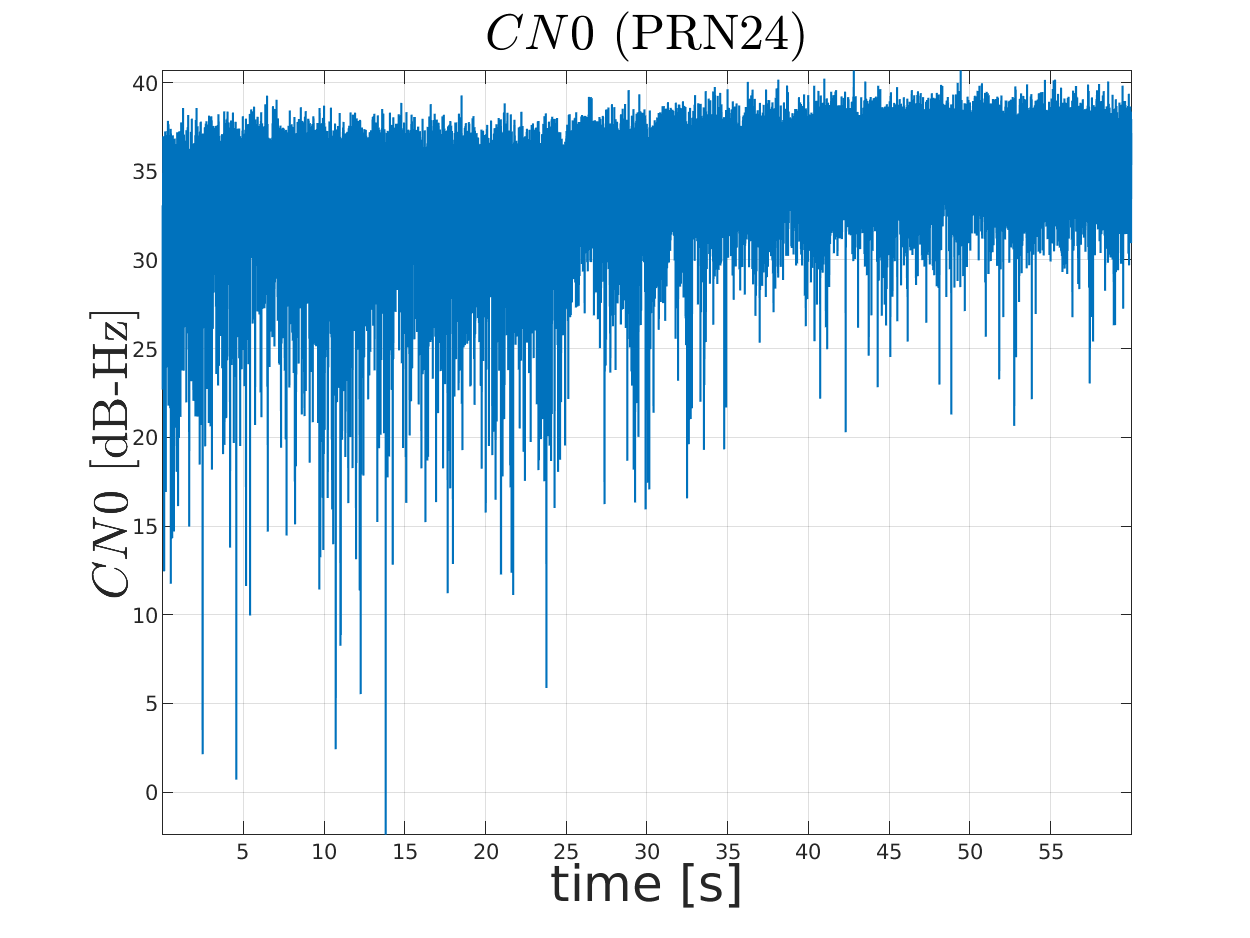
\includegraphics[width=0.9\textwidth]{fig/CN0_PRN24.png}
\end{figure}

\begin{figure}[H]
	\centering
	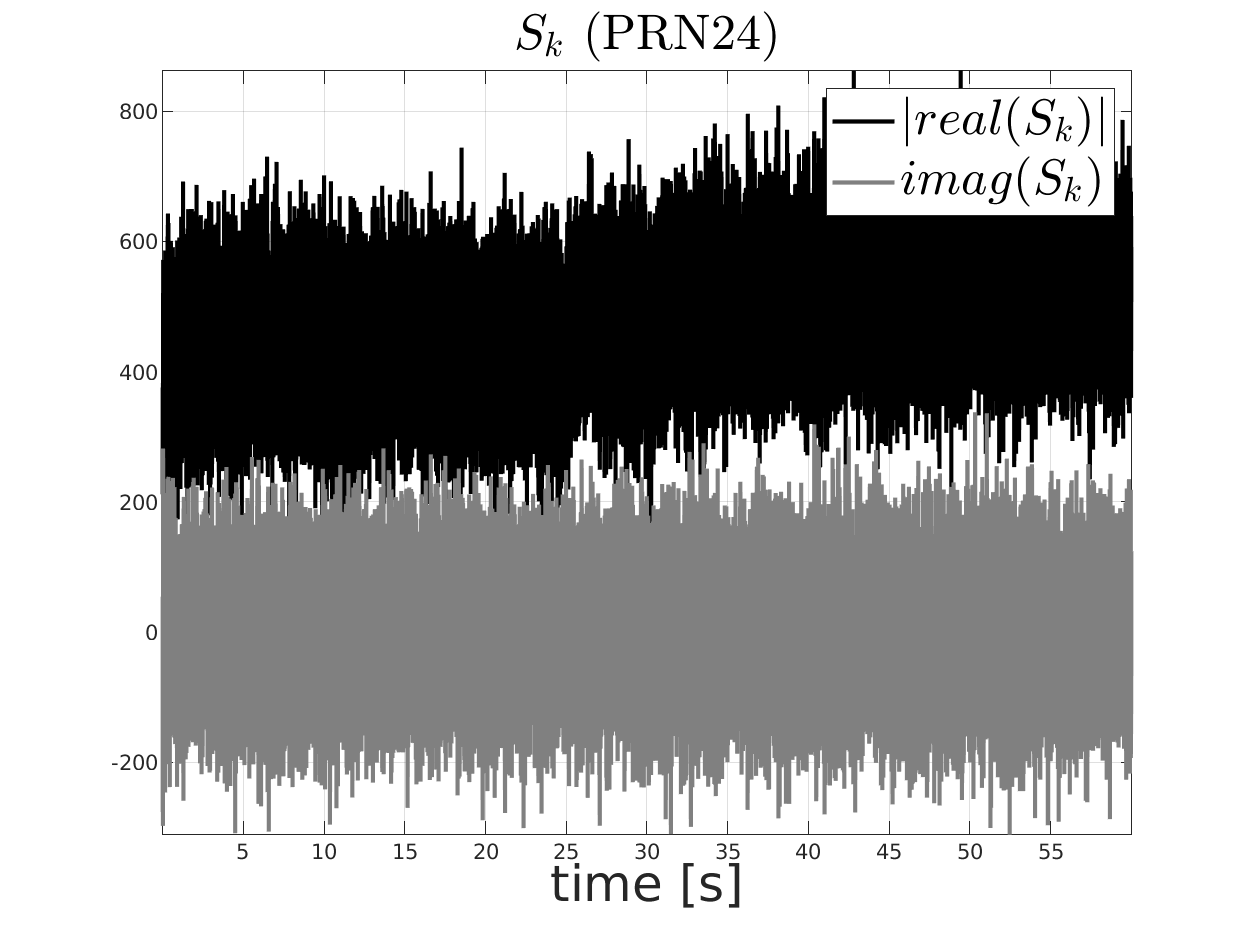
\includegraphics[width=0.9\textwidth]{fig/sk_PRN24.png}
\end{figure}

\begin{figure}[H]
	\centering
	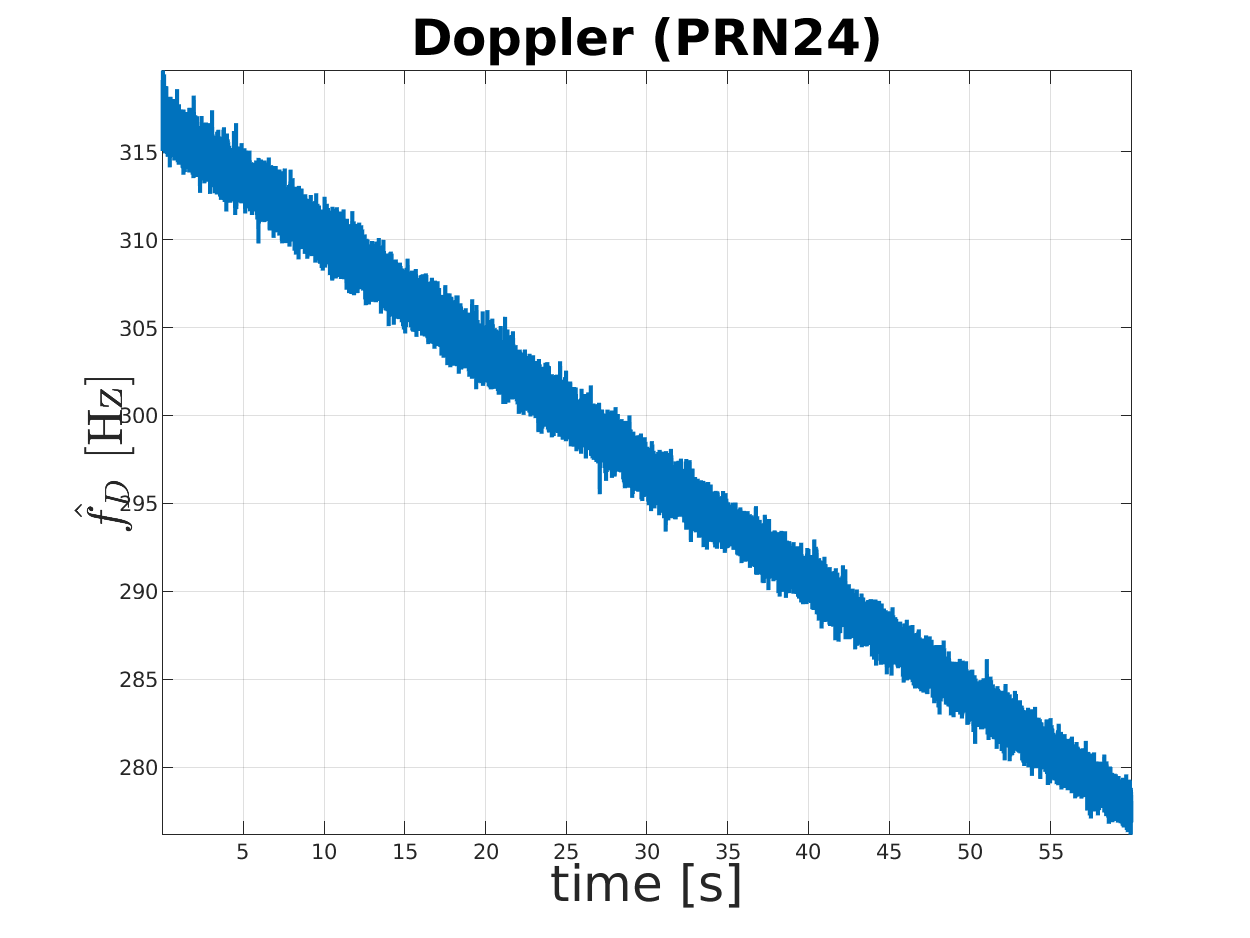
\includegraphics[width=0.9\textwidth]{fig/doppler_PRN24.png}
\end{figure}

%-------------- PRN 27
\begin{figure}[H]
	\centering
	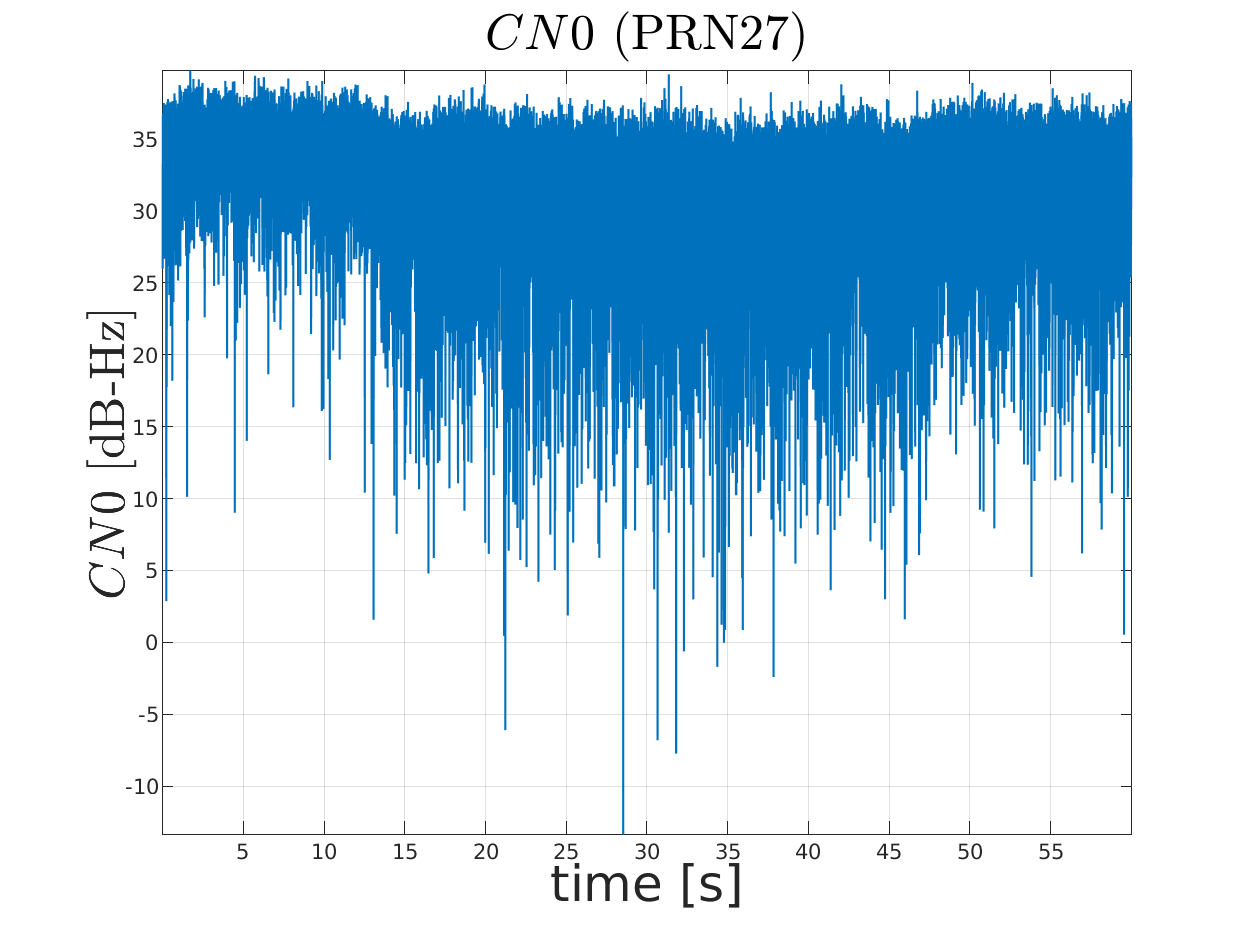
\includegraphics[width=0.9\textwidth]{fig/CN0_PRN27.png}
\end{figure}

\begin{figure}[H]
	\centering
	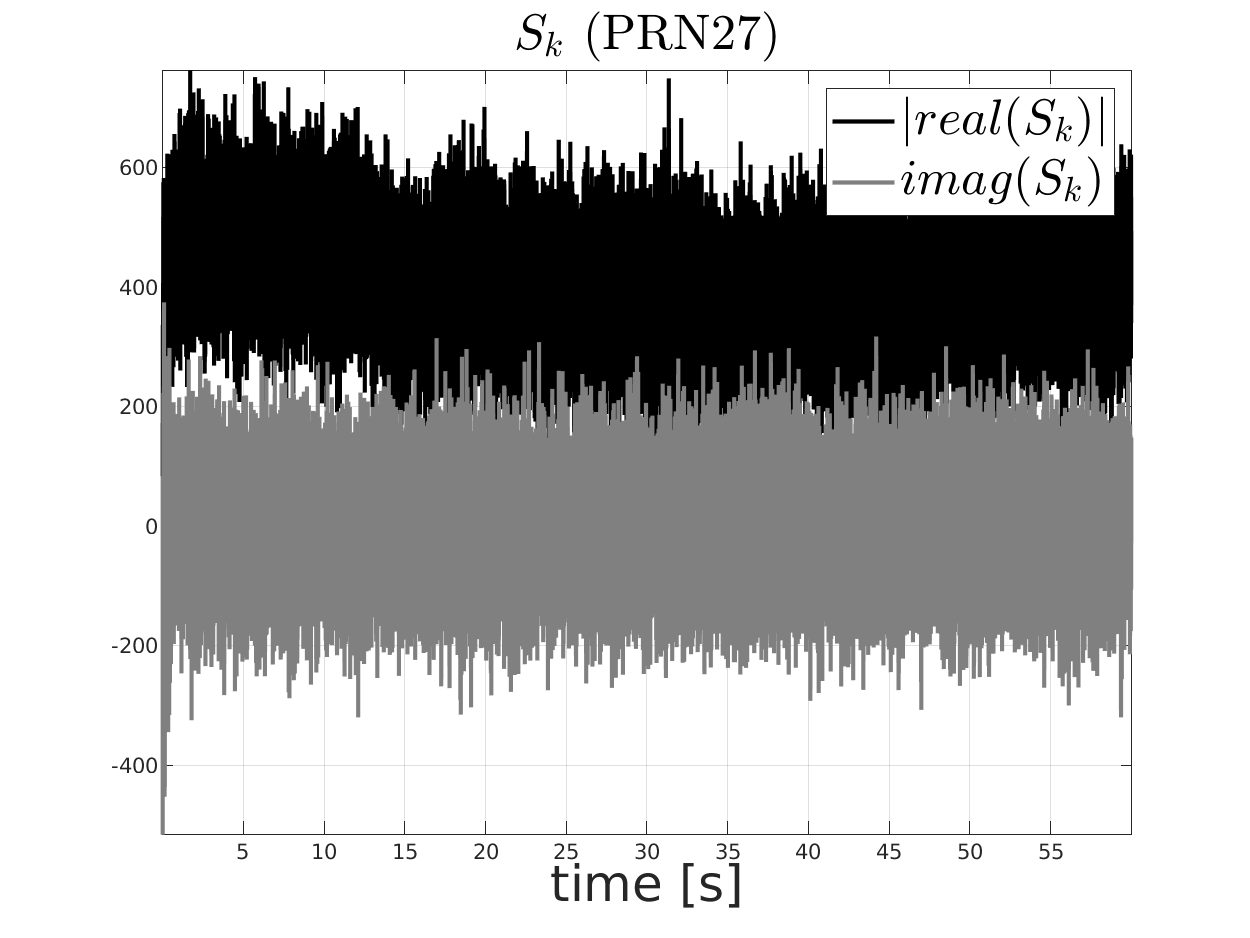
\includegraphics[width=0.9\textwidth]{fig/sk_PRN27.png}
\end{figure}

\begin{figure}[H]
	\centering
	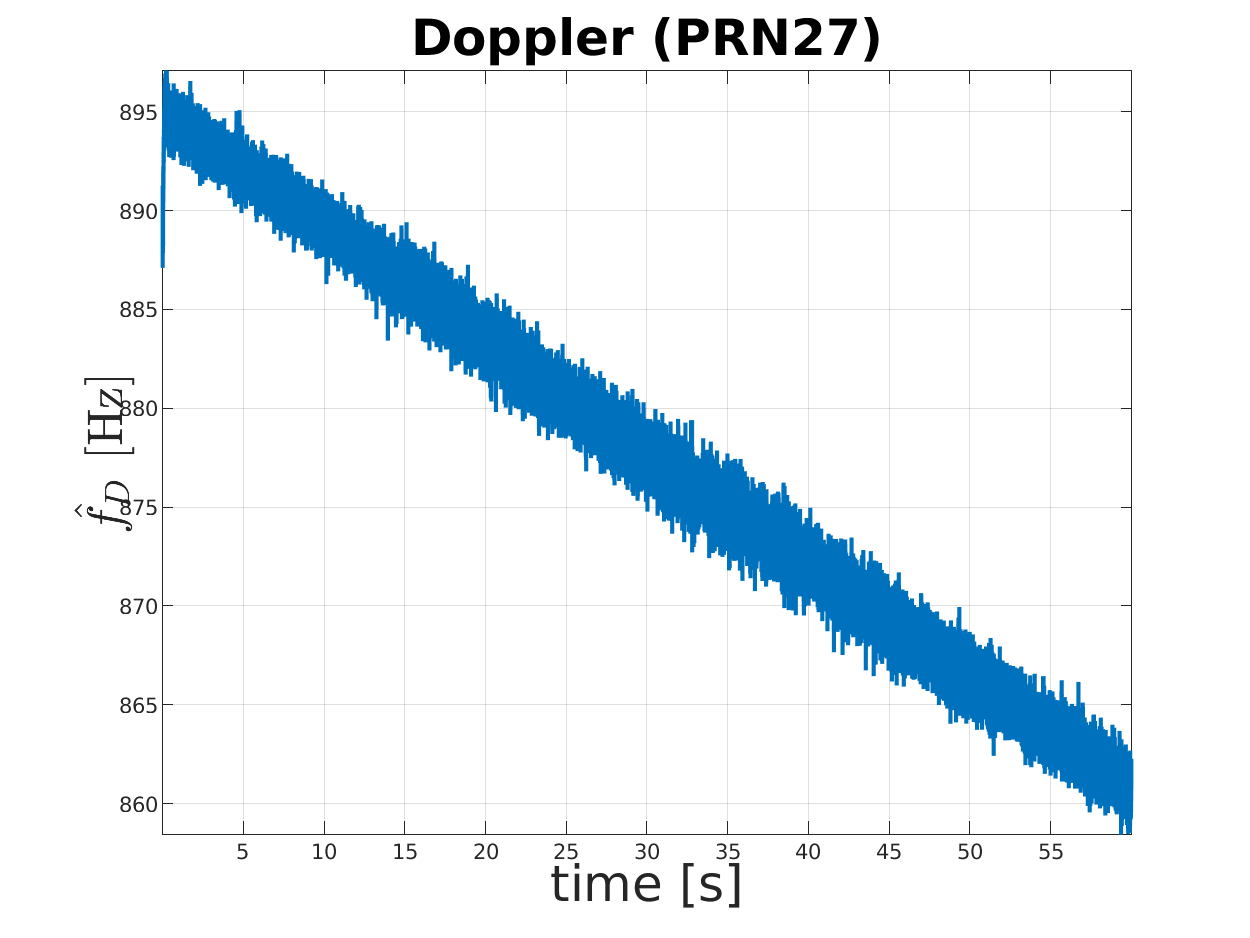
\includegraphics[width=0.9\textwidth]{fig/doppler_PRN27.png}
\end{figure}

%-------------- PRN 32
\begin{figure}[H]
	\centering
	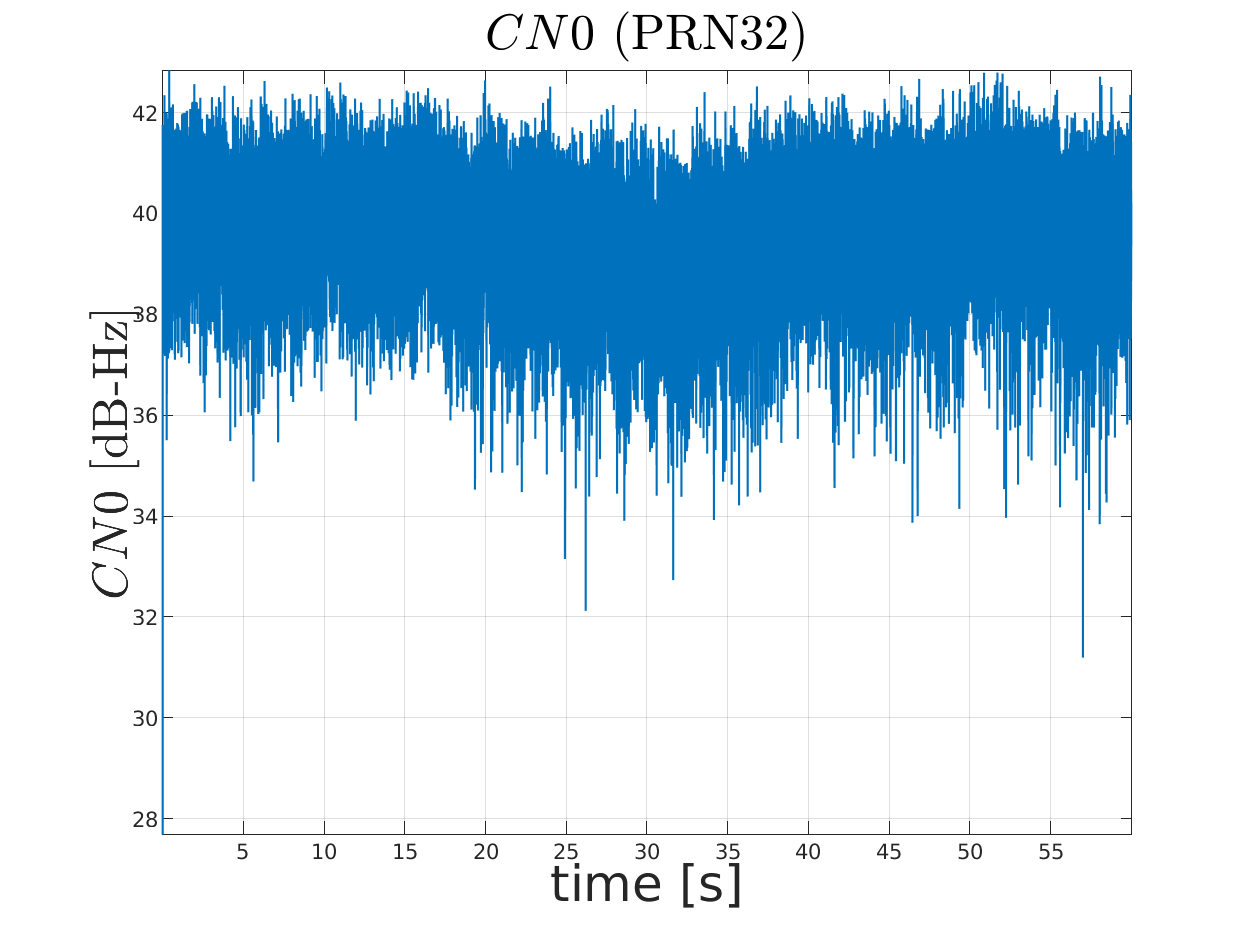
\includegraphics[width=0.9\textwidth]{fig/CN0_PRN32.png}
\end{figure}

\begin{figure}[H]
	\centering
	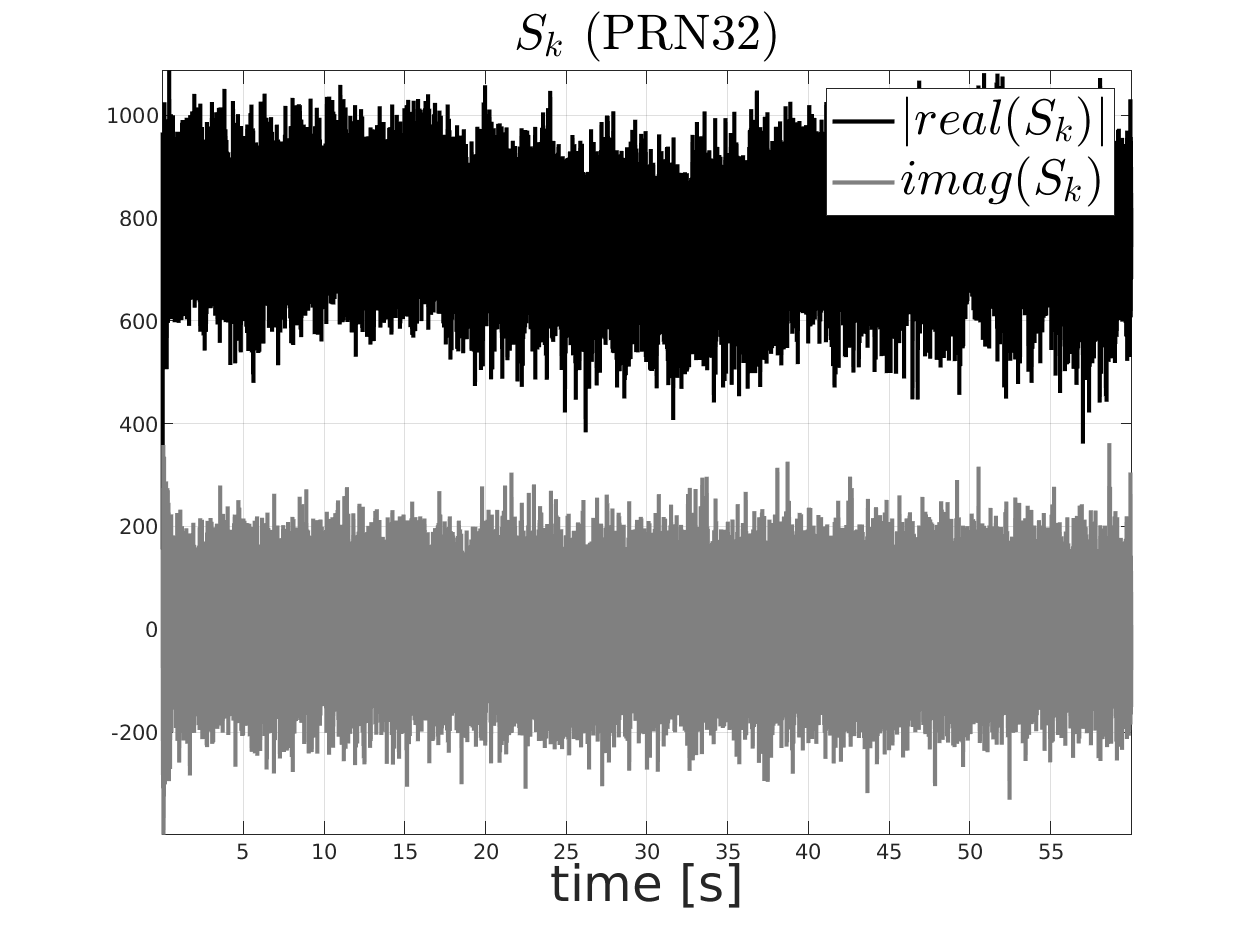
\includegraphics[width=0.9\textwidth]{fig/sk_PRN32.png}
\end{figure}

\begin{figure}[H]
	\centering
	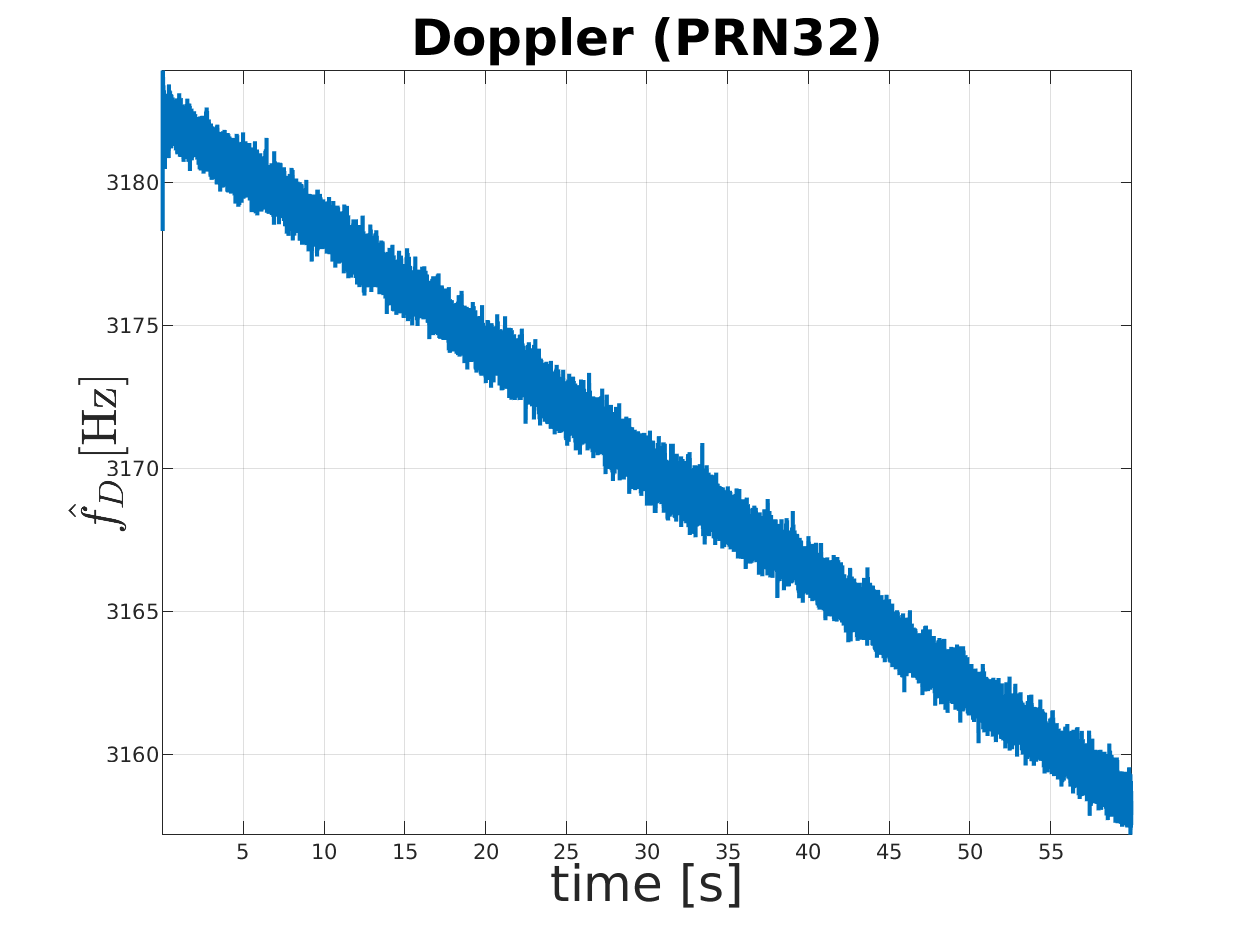
\includegraphics[width=0.9\textwidth]{fig/doppler_PRN32.png}
\end{figure}

\subsection{c}

%------------ PRN 8
\begin{figure}[H]
	\centering
	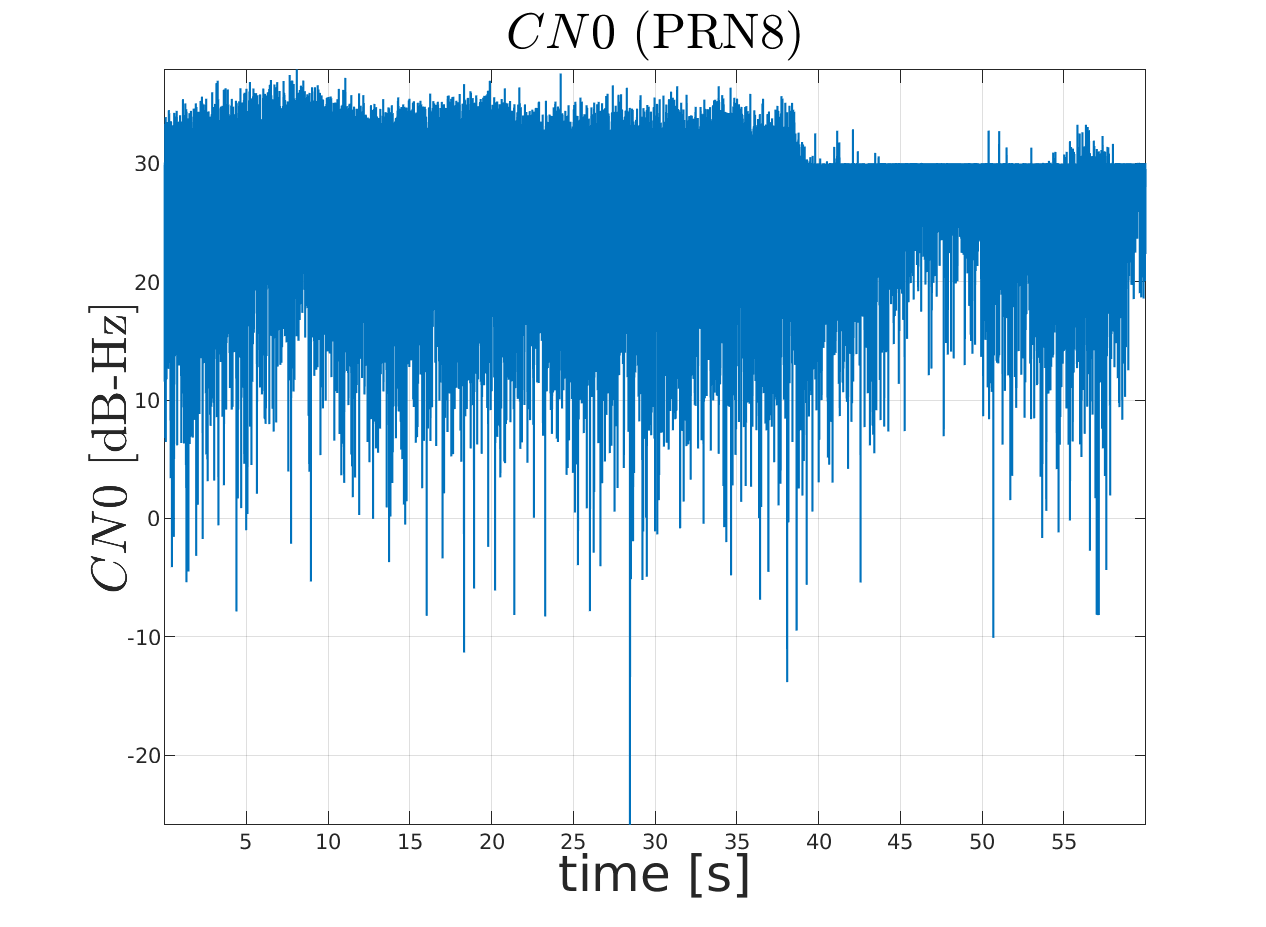
\includegraphics[width=0.9\textwidth]{fig/CN0_PRN8.png}
\end{figure}

\begin{figure}[H]
	\centering
	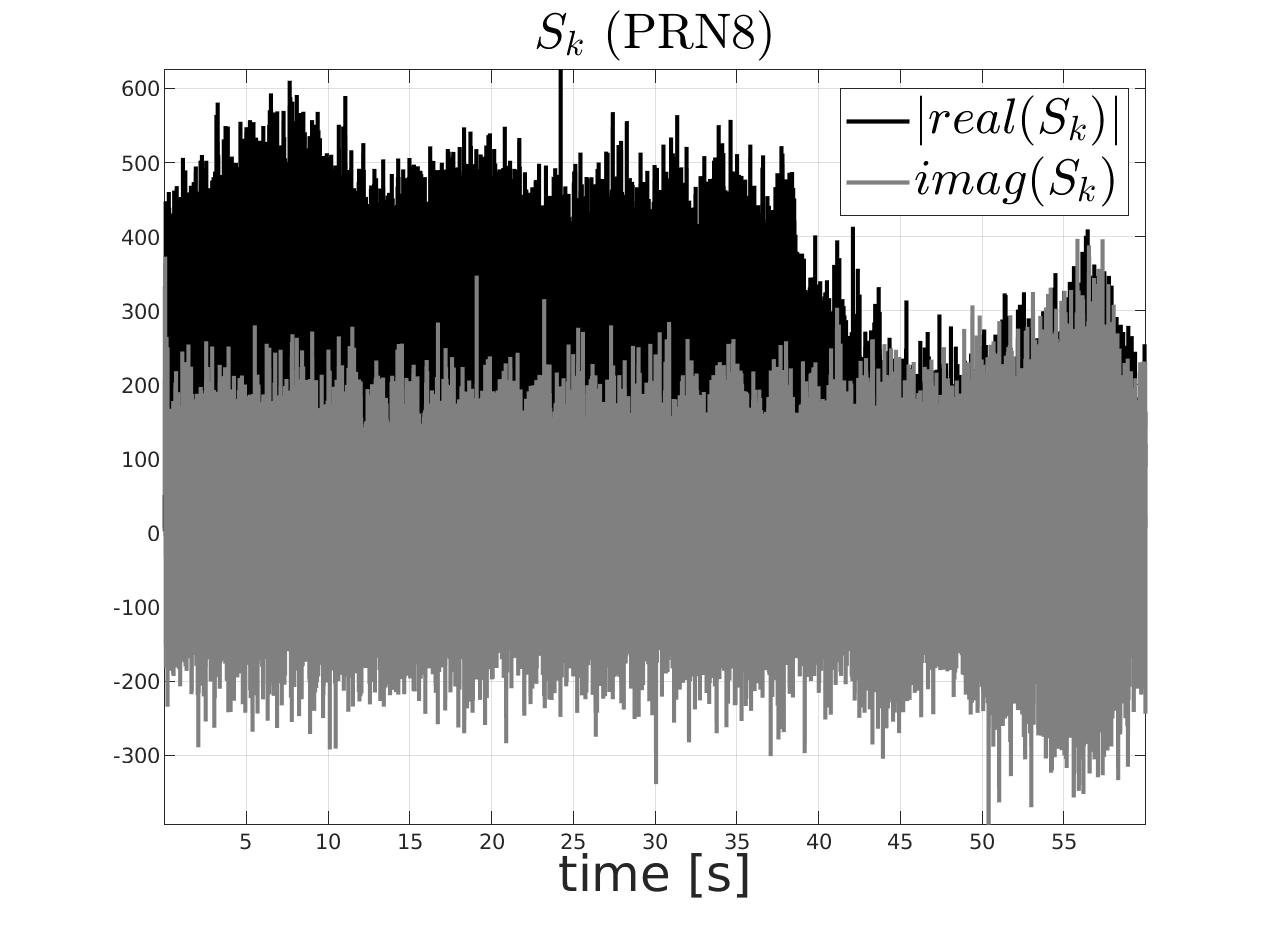
\includegraphics[width=0.9\textwidth]{fig/sk_PRN8.png}
\end{figure}

\begin{figure}[H]
	\centering
	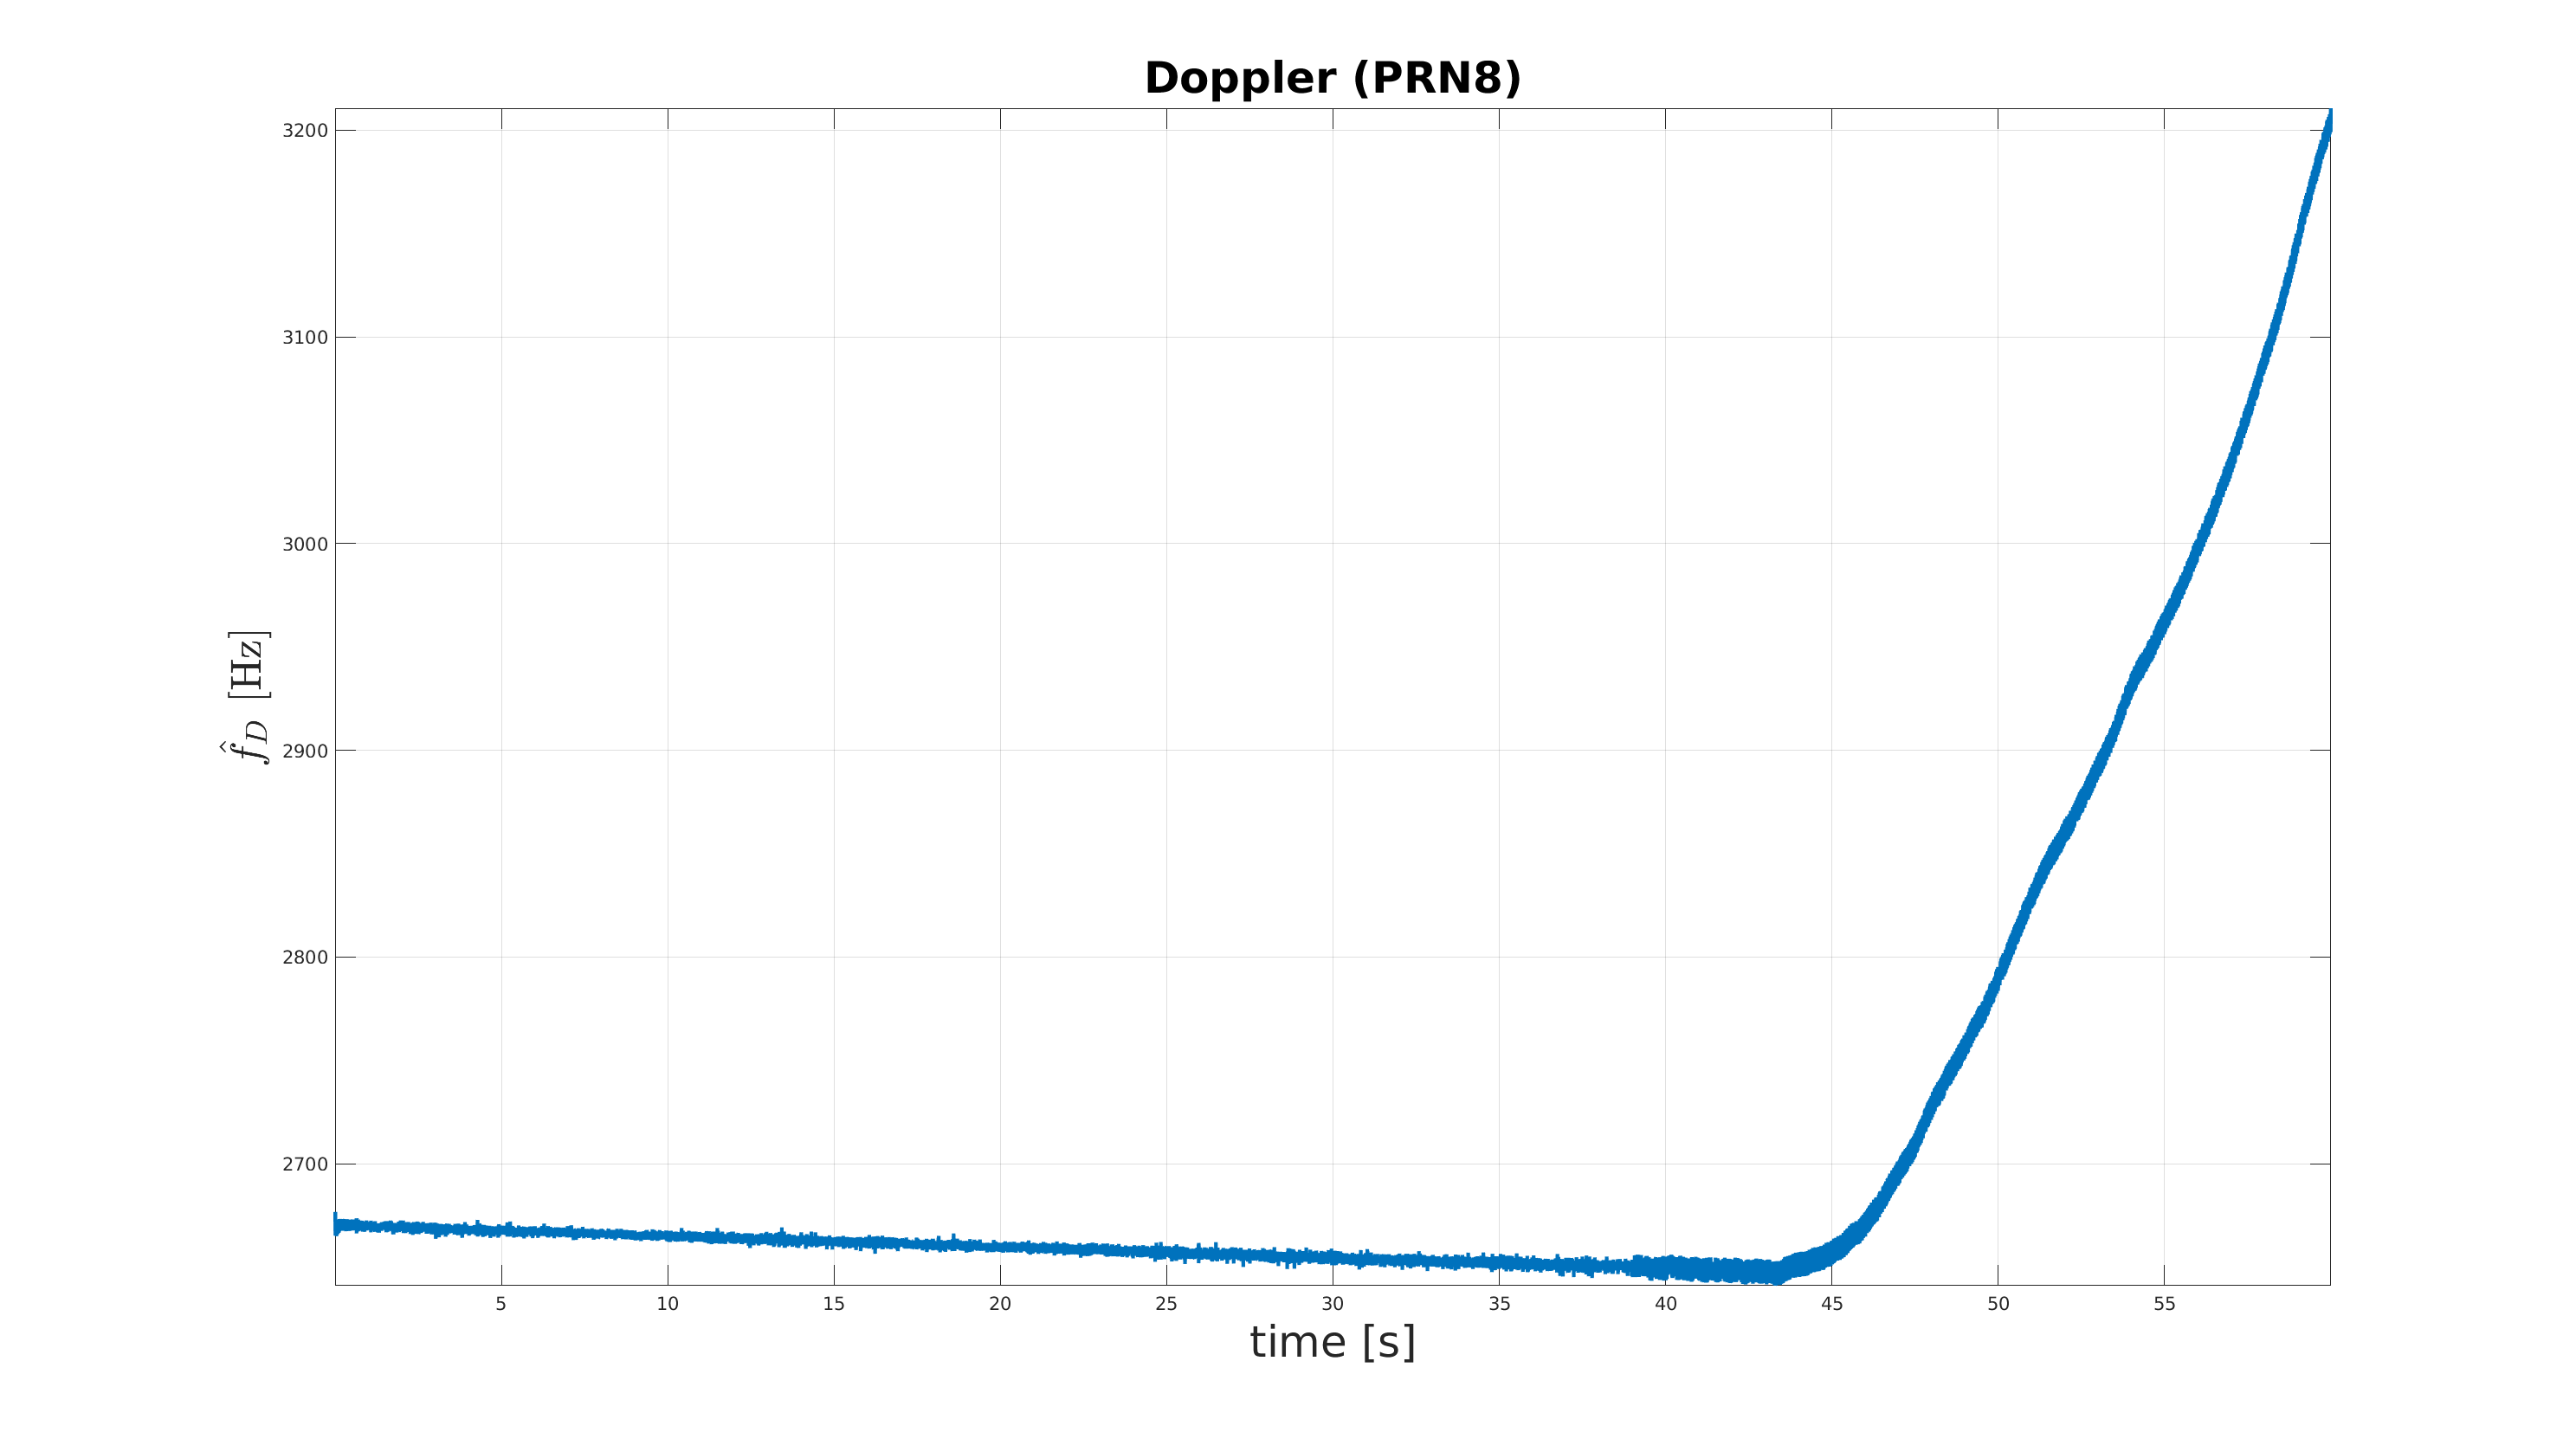
\includegraphics[width=0.9\textwidth]{fig/doppler_PRN8.png}
\end{figure}

%------------ PRN 15
\begin{figure}[H]
	\centering
	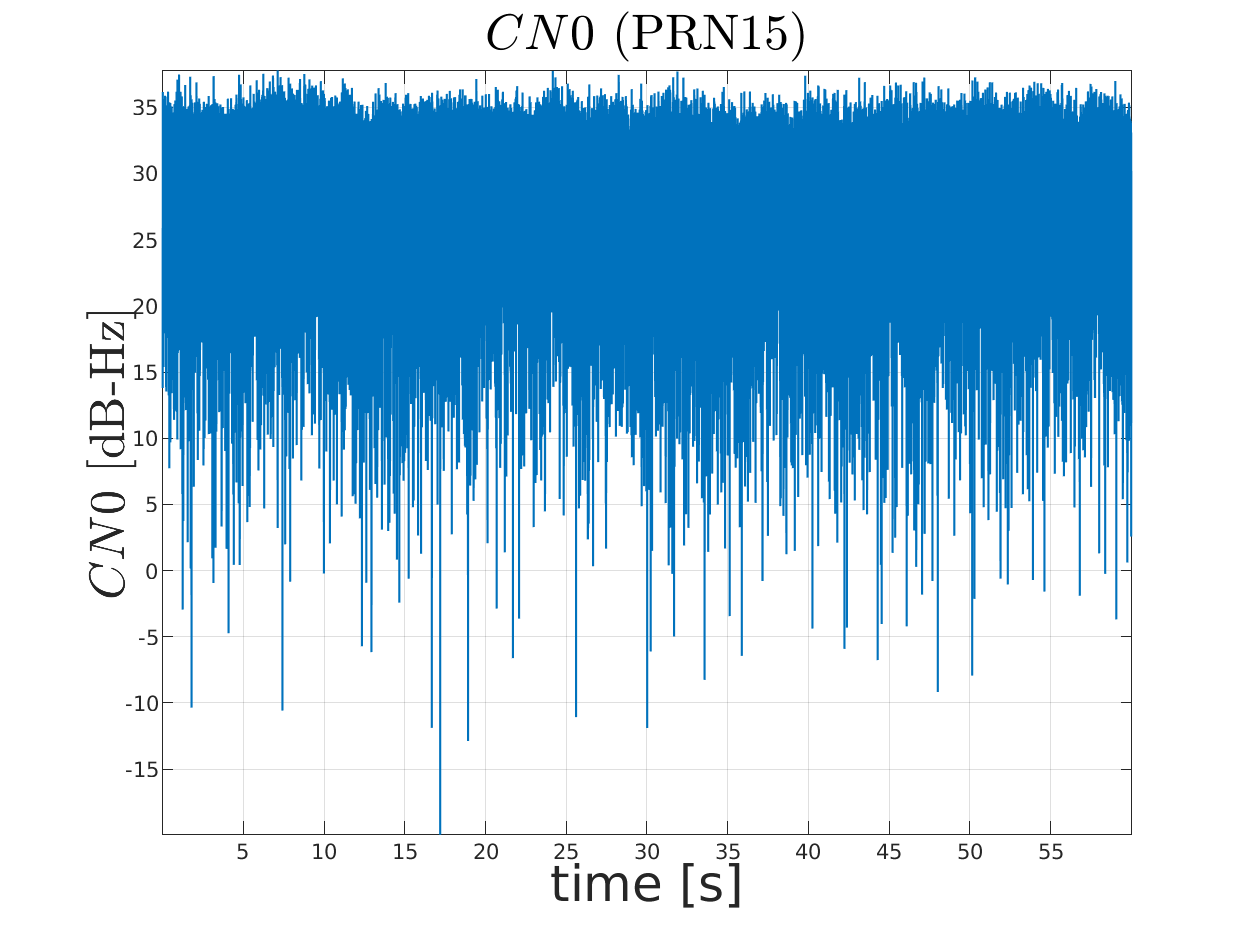
\includegraphics[width=0.9\textwidth]{fig/CN0_PRN15.png}
\end{figure}

\begin{figure}[H]
	\centering
	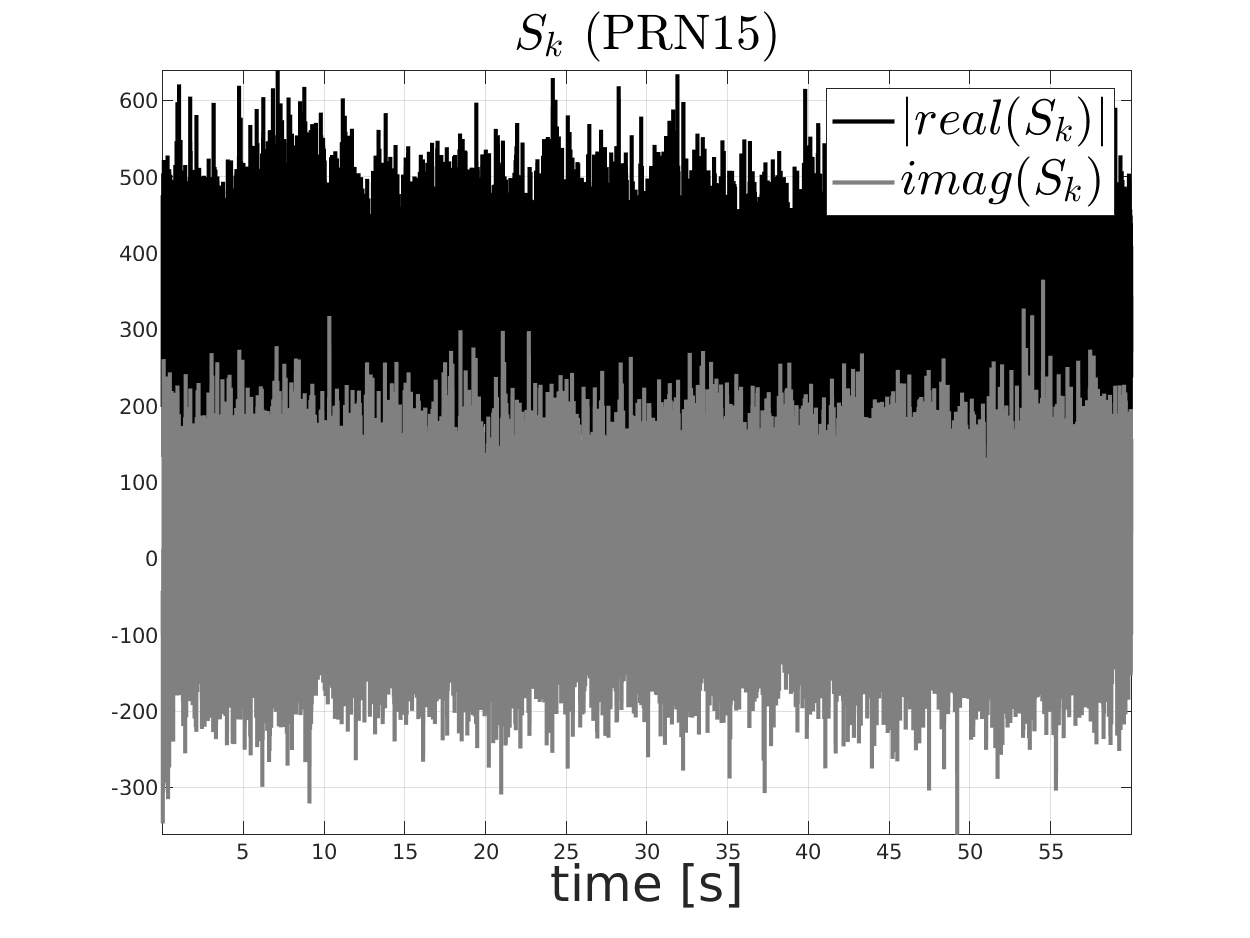
\includegraphics[width=0.9\textwidth]{fig/sk_PRN15.png}
\end{figure}

\begin{figure}[H]
	\centering
	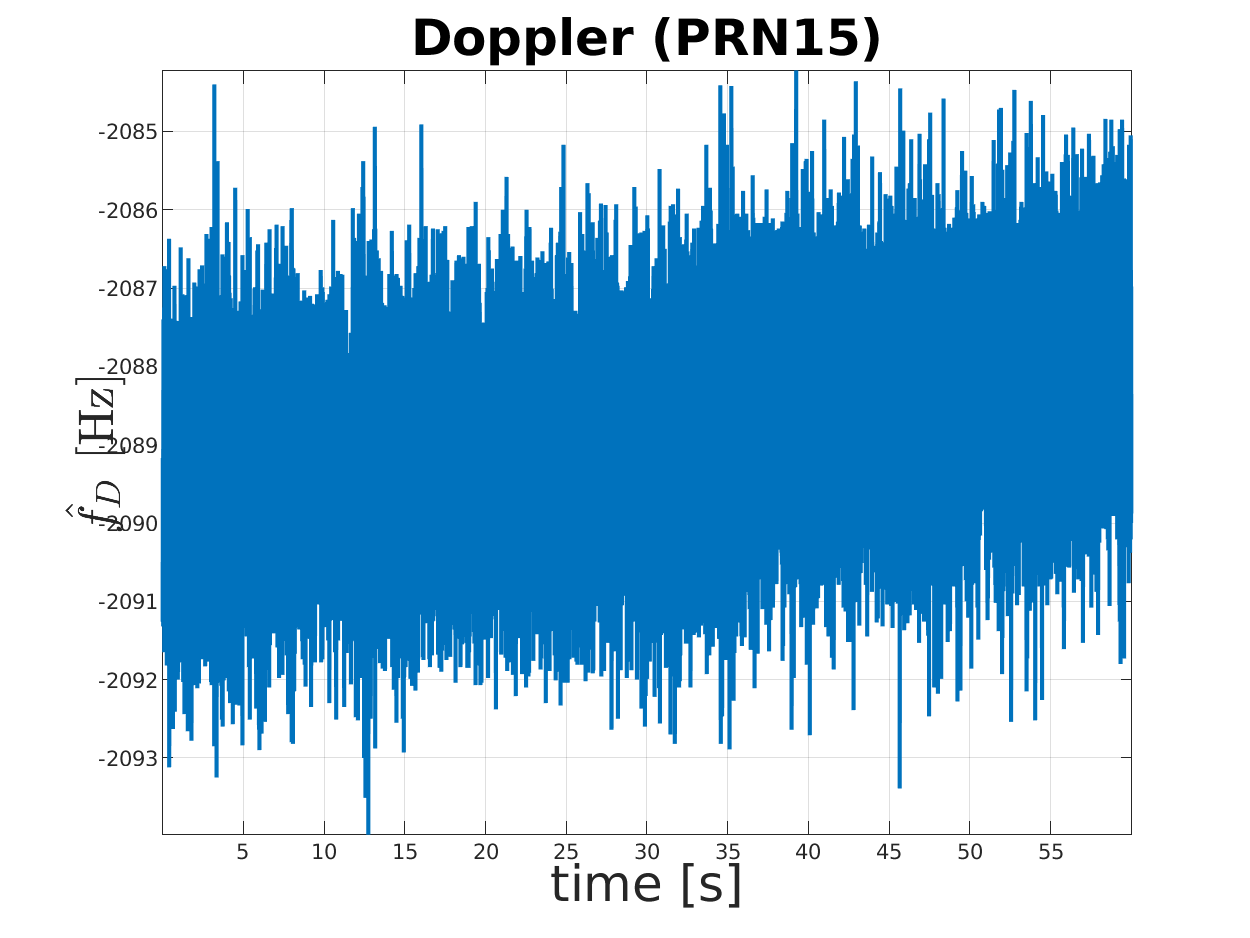
\includegraphics[width=0.9\textwidth]{fig/doppler_PRN15.png}
\end{figure}




%\bibliographystyle{ieeetr}
%\bibliography{./pangea}  
\end{document}
